%--------------------
% document principal
%--------------------

\documentclass{scrartcl}
\usepackage[utf8]{inputenc}

%\usepackage{todonotes}

%\usepackage[hmargin=2cm,vmargin=4cm,columnsep=7.5mm]{geometry}

\usepackage{biblatex}
\bibliography{bibliografia}

\usepackage[cmex10]{amsmath}
\usepackage{amssymb}

%\usepackage{graphicx}
\usepackage{tikz,pgfplots}
\usepackage{multicol}
\usetikzlibrary{dateplot}
\usetikzlibrary{shapes,arrows,positioning}
%\usetikzlibrary{dateplot}  
%\usetikzlibrary{pgfplots.groupplots}






% \pgfplotsset{
%    rrbtimeseries/.style={
%         % date coordinates in=x,
%         ylabel=Temperature (K),
%         % legend style={font=\footnotesize},
%         % tick label style={font=\footnotesize},
%         % every axis x label/.style={
%         %   at={(1.3,0)},
%         %   anchor=north,
%         %   },
%         % label style={font=\footnotesize},
%         % xticklabel style= {rotate=17,anchor=north east},
% %        every axis title shift=0pt,
% %        max space between ticks=15,
%        %  every mark/.append style={mark size=6},
%        %  major tick length=0.1cm,
%        %  minor tick length=0.066cm,
%        %  very thin,
%        %  every axis legend/.append style={
%        %    at={(1.2,0)},
%        %    anchor=south east,
%        %    draw = none},
%        % legend columns = 4,
%        % unbounded coords=jump, %v>1.4
%     },

%   % rrbrs/.style={
%   %       rrbtimeseries,
%   %       width = \textwidth,
%   %       height = 0.25\textwidth,
%   %       every axis x label/.style={
%   %         at={(1.3,-1)},
%   %         anchor=north,
%   %         },
%   %       ylabel = {},  
%   %       max space between ticks=50,
%   %       every axis legend/.append style={
%   %         at={(1,-1.1)},
%   %         anchor=north east,
%   %         draw = none},
%   %       title style={font=\small,below,anchor=north,fill=white},
%   %   },
%  }




\pgfplotsset{
   timeseries/.style={
        date coordinates in=x,
        ylabel=Temperature (K),
        legend style={font=\footnotesize},
        tick label style={font=\footnotesize},
        every axis x label/.style={
          at={(1.3,0)},
          anchor=north,
          },
        label style={font=\footnotesize},
        xticklabel style= {rotate=17,anchor=north east},
%        every axis title shift=0pt,
%        max space between ticks=15,
        every mark/.append style={mark size=6},
        major tick length=0.1cm,
        minor tick length=0.066cm,
        very thin,
        every axis legend/.append style={
          at={(1.2,0)},
          anchor=south east,
          draw = none},
       legend columns = 4,
    },
    rd/.style={
        timeseries,
        every axis x label/.style={
          at={(1.3,-1)},
          anchor=north,
          },
        label style={font=\footnotesize},
        ylabel = {},
        width=17cm,
        height=3.5cm,   
        max space between ticks=50,
        every axis legend/.append style={
          at={(1,-1.1)},
          anchor=north east,
          draw = none},
        title style={font=\small,below, at={(0.7,1.7)},anchor=north,fill=white},
    }
}


%        unbounded coords=jump, %v>1.4
%        unbounded coords=discard, %v>1.4


%http://tex.stackexchange.com/questions/46422/axis-break-in-pgfplots

%http://tex.stackexchange.com/questions/52409/insert-a-separate-mark-inside-a-pgfplots-graph


\newtheorem{definition}{Definition}
\DeclareMathOperator*{\nex}{next}
\DeclareMathOperator*{\prev}{prev}

\usepackage[bookmarks,pdfborder={0 0 0},pdfusetitle]{hyperref}

\hypersetup{
    pdfauthor={Aleix Llusà Serra; Teresa Escobet Canal; Sebastià Vila-Marta },
    pdfcreator={DiPSE--UPC},
    pdfsubject={MTSMS model},
    pdfkeywords={time series; data model; database systems; monitoring systems},
    pdflang={en},
}


\title{%
  Model and requirements for a Multiresolution Time Series
  Database Management System }


%[A. Llusà Serra; T. Escobet Canal; S. Vila-Marta]
\author
{
  {%
    A.\ Llusà Serra,
    T.\ Escobet Canal
    and S.\ Vila-Marta
  }\\
  {\{aleix, sebas\}@dipse.upc.edu, teresa.escobet@upc.edu}\\
  {Department of Electronic System Design and Programming (DiPSE)}\\
  {Universitat Politècnica de Catalunya, Manresa, ES--CT}
}



\begin{document}


\maketitle


\begin{abstract}
In this paper we define a model for multiresolution time series
database management systems. The main objective is to store compactly
a time series and manage consistently its temporal dimension. It is
achieved by extracting different resolutions and attributes summaries
from the time series.  

Our work is concerned in putting together two areas of study: time
series analysis and database management systems (DBMS). Time series analysis
offers a great deal of methodologies and algorithms to process time
series data and database field provides software expertise in managing
data. Therefore it is of primary relevance that DBMS support time series.
\end{abstract}

{\bfseries Keywords:} time series, data model, database systems,
monitoring systems.


%\twocolumn

%intro, requirements



\section{Introduction}



Information collection processes are growing in quantity as a
consequence of the emergence of embedded systems and sensor networks.
Nowadays it is possible to collect large amounts of data to monitor
and control complex systems.  This information must be analysed and
prepared by information systems in order to detect eventual sensor
failures or malfunctions and, if it is possible, to reconstruct the
incorrect signals. Acquired data instance are bound to a timestamp,
therefore correctness criteria must include both data value and its
timestamp. The sequences of data values collected at specific
timestamps are formalised as time series.


Time series are defined as a collection of observations made
chronologically.  In general, time series come from a continuous
nature in which they are recorded at regular intervals, such as hourly
or daily, or at irregular intervals, such as recording when a pump is
open or closed.  One problem when dealing with time series data
results from the fact that these data are often voluminous
\cite{fu11,keogh08:isax}, as a result, efficiently storing and
accessing them can be complex. Moreover, this is specially critical
when developing small embedded systems, whose resources (capacity,
energy, processing and communications) suffer restrictions
\cite{yaogehrke02}.  Another problem is that the procedure of
processing and synthesising information becomes difficult if data is
not equi-time spaced.



Time series can be stored and managed by Structured Query Language
(\acro{SQL}) relational database management systems. However, some
authors \cite{dreyer94,schmidt95,stonebraker09:scidb,zhang11} notice
that the use of \acro{SQL} systems as a time series backend suffers
some drawbacks.  On the one hand, \emph{NoSQL} or \emph{NewSQL}
products are being developed in order to increase the performance and
flexibility of \acro{SQL} systems
\cite{atzeni13:relational_model_dead,stonebraker10,stonebraker09:scidb,zhang11},
however the continue acquisition nature of time series is an issue for
storing and analysing offline all the data \cite{keogh97}.

On the other hand, compression techniques for time series are
considered in the form of approximation to the original signal in
order to compute analysis such as similarity or pattern search
\cite{fu11,keogh01,last01} or in the form of compression and
aggregation approaches for massive data streams
\cite{cormode08:pods,bonnet01}. However, treating time series as data
streams does not consider adequately the time dimension nor computes
the evolution of aggregated parameters along time, which is
interesting for monitoring purposes.  On a similar approach,
\emph{RRDtool} \cite{rrdtool} is a system that stores time series
aggregated in different resolutions in order to compact data and to do
faster visualisations. However, \emph{RRDtool} is very specific and
has limited aggregation operations to applications of network
counters.



\subsection{Contribution}


%TSMS

This paper focuses on Data Base Management Systems \linebreak[4]
(\acro{DBMS}) that store and treat data as time series, usually known
as Time Series Data Base Management Systems (\acro{TSMS}),
\cite{dreyer94,last01}.  We introduce a new data model named
multiresolution \acro{TSMS} (\acro{MTSMS}). This model organises data
in an aggregated way and  allows to store time series using
different time resolutions. It is designed to cope well with bounded
storage computers such as sensor systems.  

We describe the model in two separated submodels, one \acro{TSMS}
model mainly for describing time series basic concepts and operations
and the other a \acro{MTSMS} model for describing multiresolution over
time series. The model is described firmly rooted on set and
relational algebra as a formal theory for information systems.  It
also considers the time irregularities sampling of time series,
moreover it operates coherently with the time dimension of time
series.


% Our multiresolution definition is
% based on concepts of RRDtool but aims to generic applications and has
% more generic operators.


Multiresolution is proposed as a lossy storage solution that selects
only the needed information. The concept is similar to multimedia
lossy compression methods, where information can be discarded in
favour of size, but applied to time series.  Multiresolution is an
aggregation of data that stores the evolution of the parameters along
time, which is more related to the needs of monitoring. However, as a
lossy storage solution, the multiresolution schema has to be decided
for each application, deciding what approximate queries will be needed
to resolve. We formalise aggregation functions as an independent
object of the main model. Therefore, users can define new operations
and other aggregation methods from other fields such as data
streaming or time series data mining.


A representation function concept of time series is also formalised, then
users can define different operators considering the behaviour of time
series in different contexts. Especially, it is important when defining
new aggregation operations that must consider different meanings of
the time series, i.e. \emph{RRDtool} specific counter time series
aggregations. Furthermore, we formalise representation as an
independent object of the main model.




\subsection{Outline}

This manuscript is organised as follows.  In
Section~\ref{sec:related-work} some related work concerning
\acro{TSMS} and \acro{MTSMS} are presented.  The motivation for
multiresolution is shown in Section~\ref{sec:features}.  The
\acro{TSMS} model is presented in Section~\ref{sec:model:TSMS} and the
\acro{MTSMS} model is presented in Section~\ref{sec:MTSMS}.  In
Section~\ref{sec:implementation} there is a implementation
for the \acro{TSMS}+\acro{MTSMS} model.  Section~\ref{sec:example} is
devoted to a real data multiresolution database example.  Finally,
Section~\ref{sec:concl-future-work} offers some conclusions.
\ref{sec:notation} shows main notation symbols.





\section{State of the art}
\label{sec:related-work}

In this section, related work to mutiresolution time series is
described in three parts: some database management systems
approaches for time series, compression techniques applied to time
series, and computations based on data streams.




\subsection{Database approaches}

Some authors treat \acro{TSMS} as a particular \acro{DBMS} field
\cite{last01}.  Segev and Shoshani \cite{segev87:sigmod} propose an
structured language for querying \acro{TSMS}. Their time series
structures include the notion of regularity and temporal
representation and their operations are \acro{SQL}-like.  Dreyer et
al.\ \cite{dreyer94} propose the requirements of special purpose
\acro{TSMS} and base the model on five basic structural elements:
events, time series, groups, metadata and time series bases. They
implement a \acro{TSMS} called \emph{Calanda} which includes calendar
operations, allows grouping time series and operating with simple
queries. They exemplify it with financial data. In \cite{schmidt95}
\emph{Calanda} is compared with temporal systems designed for time
series.



 
Others implement \acro{TSMS} with array database approaches.
\emph{SciDB} \cite{stonebraker09:scidb} and \emph{SciQL}
\cite{zhang11} are array database systems intended for science
applications, in which time series play a principal role. They
structure time series into arrays in order to achieve multidimensional
analysis and they store other data into tables.  \emph{SciDB} is based
on arrays which, according to the authors, allow to represent time
series.  In contrast, \emph{SciQL} defines time series as a mixture of
array, set, and sequence properties and exhibits some time series
managing characteristics that include time series regularities,
interpolation or correlation queries.
% However,
% difference between tables and arrays seems too physical and leads to
% ambiguity when representing time series.  
% Our TSMS model proposes time
% series as firmly based on relational algebra, clarifying this
% ambiguity and describing them coherently in terms of information
% systems theory.





Bitemporal \acro{DBMS}, sometimes referred directly as temporal data,
is a database field related with time. Bitemporal data manages
historical data and events in databases by associating pairs of
\emph{valid} and \emph{transaction} time intervals to data.
Bitemporal data and time series data are not exactly the same and so
can not be treated interchangeably \cite{schmidt95}, however, there
are some similarities that can be considered. Moreover, \acro{DBMS}
research represents bitemporal data as relations extended with time
intervals attributes and extends relational operations in order to
deal with related time aspects
\cite{jensen99:temporaldata,date02:_tempor_data_relat_model}.  We
formalise time series similarly as how bitemporal data is formalised
for relational \acro{DBMS}.
% On the other hand, some bitemporal time concepts might be taken
% into account by \acro{TSMS}, such as the discussions about time
% granularities.



\subsection{Compression techniques}


% As \acro{TSMS} suffer from problematic properties of time
% series, like the ones we describe in
% Section~\ref{sec:model:properties} mainly the huge data volume,
% compression techniques are used.  Next, we summarise some current work
% in \acro{TSMS} with compression.



\emph{RRDtool} from Oetiker, \cite{rrdtool,lisa98:oetiker}, is a free
software database management system. It is designed to be used for
monitoring systems. Because of this, it is focused to a particular
kind of data, gauges and counters, and it lacks general time series
operations. \emph{RRDtool} can store multiple time resolution data,
however Plonka et al.\ \cite{lisa07:plonka} evaluated \emph{RRDtool}
performance and found limitations when storing huge number of
different time series. They propose a caching system on top of
\emph{RRDtool} as a solution.  \emph{RRDtool} is extremely used by the
free software community so it inspired us to develop a model from its
main characteristics, that is now what we call multiresolution. A
similar approach is done by \cite{weigel10} in a system called
\emph{TSDS} that caches queries by aggregate parameters. They notice
that data needs to be shown over its full time range and not only
subsets of data as it is usually provided.  They develop the software
package \emph{TSDS} where time series are stored fully and then
requested by date ranges or by applying different filters and
operations to the time series data.  Our \acro{MTSMS} model is a generic
approach to the multiresolution features, we define it open so that
users can define any attribute aggregate functions.


Deri et al.\ \cite{deri12:tsdb_compressed_database} present
\emph{Tsdb}, a lossless compression storage \acro{TSMS} for time
series that share the same time instants of acquisition. Different
time series are stored grouped by the time of acquisition instead of
each time series isolated.  They compare \emph{Tsdb} with \emph{RRDtool} and
with a relational product. As a consequence of \emph{Tsdb} structure,
they achieve a better measure addition time but a worse global
retrieval time as data has to be contiguously regrouped. However, when
measures have same time this is seen as the same time series in a
\acro{MTSMS}, so it would be interesting to use this implementation
architecture of shared time arrays in \acro{MTSMS} for resolution subseries
with same delta time in order to achieve better performance requirements
when having much equal acquired time series.

% Therefore, as it is a very different approach from RRDtool we find it difficult to compare both in these performance requirements. 
% He only evaluates compression performance but we think that a global
% evaluation of compression plus descompression must be done. MTSMS
% are not aimed to be a replacement for offline long time storage
% systems that are rarely queried and then queries can be slow but
% have tot be exact. MTSMS are adequate to stream processing and
% resolving queries with less data than original and so they are
% quicker but give information previously selected.


There are other lossy compression techniques for time series devoted
to the optimal approximation representation, that is finding the
compromise between least data that can reconstruct the original signal
with least error. Keogh et al.\ \cite{keogh01} cite some possible
approximation representations for time series such as Fourier
transforms, wavelets, symbolic mappings or piecewise linear
representation. They remark this last one as very usual due to its
simplicity and develop a system called \emph{iSAX}
\cite{keogh08:isax,keogh10:isax} in order to analyse and index massive
collections of time series. They describe that the main problem is in
the indexing of time series and they propose methods for processing
efficiently. The first method proposed is based on a constant
piecewise approximation. The time series representation obtained with
\emph{iSAX} allows reducing the stored space and indexing faster with
the same quality as other more complex representation methods.  These
compression techniques are candidates for being used as attribute
aggregate functions in the \acro{MTSMS} model, as instance it would be
interesting to define aggregations in the frequency domain of time
series.


% A Multiresolution Symbolic Representation of
% Time Series; Megalooikonomou, Faloutsos; 2005 proposes multiresolution by decomposing a signal in frequency subsequences and intended mainly to similarity searching. The objective is to reconstruct the original time series. 
 


% \paragraph{T-Time}  \textcite{assfalg08:thesis} shows a TSMS that can do similarity search, which is calculated as distances between time series. Mainly, two time series are marked as similar if they distance is less than a threshold in each interval. From this method efficient algorithms are developed and implemented in a program called T-Time, which is described in \cite{assfalg08:ttime}.

 


\subsection{Data stream}



There are other \acro{TSMS} specifically designed for a particular
field requirements.  \emph{Cougar} \cite{bonnet01} is a sensor
database system that has two main structures: one for sensor
properties stored into relational tables and another for time series
stored into data sequences from sensors. Time series have specific
operations and can combine relations and sequences. \emph{Cougar}
target field is sensor networks, where data is stored distributed in
different locations. Queries are resolved combining sensor data in a
data stream abstraction that improves processing performance.

Time series as data streams are also considered when aggregating
statistically data in order to do fast approximate queries with
compressed data, Cormode et al.\ \cite{cormode08:pods} develop
aggregation techniques that consider giving more weight to recent
information.  Our \acro{MTSMS} model applies a similar approach of
weighting more recent data but specifically to time series, with
multiple aggregations and considering time irregularities.


% Our MTSMS model can also be thought as an stream processor if measures
% are added in time order, there is no possibility of update operations,
% buffer time series become of unity cardinality, and aggregate
% functions are limited to stream capabilities ones.  
% As instance,
% RRDtool can be considered stream oriented and its consolidation
% process is done at the same time of inserting new measures.





\section{Multiresolution motivation}
\label{sec:features}

A \acro{TSMS} is a special purpose \acro{DBMS} devoted to store and
manage time series.  The main objective of \acro{TSMS} is to gather
two areas of study: time series analysis and \acro{DBMS}.  Time series
analysis formalises a great amount of algorithms and methodologies
that apply to time series, with a main focus on improving
efficiency. \acro{DBMS} theory formalises systems that store and
operate with data, currently the relational model is the referent
\cite{date:introduction}.



In time series analysis there are some common generic operations.
Most of these operations deal with the time given the nature of data.
Usual operations include querying time intervals, finding time
correlations, or calculating distances between two time series. In
all these operations \acro{TSMS} must consider the temporal coherence
of the time series.  In the context of statistics, aggregation of time
series is also a common operation. Aggregate means to summarise a time
series subset by a smaller set of measures. Statistic indicators like
the mean, the maximum, or the mode, for instance, summarise time
series into one only measure.

In the discrete context, a time series is defined as a set of value
and time pairs. Furthermore, a time series has a continuous nature as
it comes from a phenomena evolution along time. As a result,
\acro{TSMS} operations may deal with this time series nature by
methods of interpolation or approximation.


A \acro{MTSMS} proposes a \acro{TSMS} with multiresolution
capabilities.  A \acro{MTSMS} schema represents a time series using a
set of different resolutions.  The multiresolution concept comes from
thoroughly analysis of \emph{RRDtool} \cite{rrdtool}. Our objectives
have been to formalise the main concepts into an abstract model and to
include more genericity in order to describe \acro{MTSMS} as fully
\acro{TSMS}.

%Then we will be able to apply these systems to other applications.

As a summary, \acro{MTSMS} improve \acro{TSMS} features in various aspects:
\begin{itemize}

\item Voluminous data. Monitoring systems capture a huge amount of
  data from sensors. In order to be able to process this information,
  data volume must be reduced. One of the features of the
  multiresolution approach is to select and store only the most
  interesting segments of data. This segments are seen as different
  resolutions for the same time series and the user can configure how
  they are extracted and summarised by defining different time steps
  and functions. Multiresolution can also be useful when graphing time
  series allowing the user to select the best time range and time
  step that fits into the screen; there is no need to process with
  more quantity of data than the one that can be
  shown.% In figure~\ref{fig:mtsms:sequence} there is an example of
  % extracting two resolutions: one every three units of time and
  % another every five.

\item Data validation. Monitoring systems capture data but can occur
  some drawbacks that will affect later the process of time series
  analysis. Main problems are found when monitors can not capture
  data, known as gaps, or capture data erroneously, such as outlayers
  \cite{quevedo10}.  The multiresolution attribute functions is
  designed to cope well with validating, filtering and reconstructing
  with this unknown data in order to keep a consistent
  historic.% In figure~\ref{fig:mtsms:sequence-irregular} an
  % example of a gap can be seen.

\item Data time regularising. Another monitoring side effect happens
  when the sampling rate is not constant, that is when the resulting
  data is not equi-time spaced. This no regularities can come from
  sampling jitters in periodic sampling or from no periodic
  event-based sampling \cite{kopetz11:realtime}. One multiresolution
  consolidation objective is to regularise the time interval when
  processing a time series, therefore each resulting time series
  segment has a regular time resolution. This regularising approach
  could also be used when the user wants to consult another resolution
  for a time series, such as changing periodic data from a month to a
  year step. % In
  % figure~\ref{fig:mtsms:sequence-irregular} an example of time
  % regularising can be seen.

\item Information summaries. Time series analysis typically focuses on
  reconstructing the original signal. However, the user objective in a
  database system is to consult some information. The multiresolution
  approach allows a lossy compression storage solution for data. Therefore
  it can be regarded as to extracting the interesting information and
  then storing it. The selected information must be determined a
  priori assuming the context where the future queries will be done.
  % In
  % figure~\ref{fig:mtsms:sequence} there is an example of summarising by
  % mean attribute.
\end{itemize}


However sometimes it may also be useful to complement \acro{MTSMS}
with other \acro{DBMS}. Not only to store the original values as a
long-term deposit consulted offline, but also to store related
information to time series such as units of values, sensor
localisation, classification tags, last measured value, etc.



\subsection{Motivation example}
%We give a motivation example of multiresolution applied to a time series.  

Figure~\ref{fig:mtsms:sequence} shows an example of a multiresolution
summary for a time series. It shows a snapshot in time, suppose
between time 9 and 10. At the top of the figure there is a plot of a
time series with time axis in general units of time (u.t.) and with
value axis in undetermined units. The 'now' point shows when the
snapshot has been taken, so the time before is the past and the time
after is the future, which is grey coloured. The \emph{init} point
shows when the database system has started sampling, so data in time
before is unknown; the starting point is indicated as zero u.t.\ and
the earlier unknown time points have negative units.


\begin{figure}
  \centering
  %\usetikzlibrary{positioning}
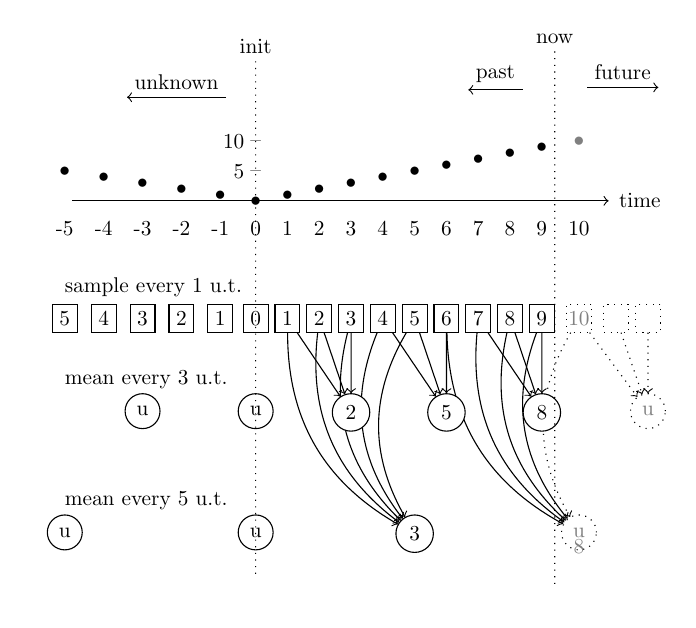
\begin{tikzpicture}[scale=0.77, every node/.style={transform shape}]

  %referencia
  \node (-6) {};

  \foreach \x in {-5,...,12}
  {
    \pgfkeys{/pgf/number format/.cd,int trunc}
    \pgfmathparse{abs(\x)}
    \let\absx=\pgfmathresult
    \pgfmathparse{\x-1}
    \let\antx=\pgfmathresult
    %time
    \node[node distance=1mm] (\x) [right=of \antx] 
    {\ifnum\x<11 \x \else \phantom{9} \fi};

    %graph values
    \node [above=\absx mm of \x] 
    {\ifnum\x=10 \color{gray} \fi \ifnum\x<11 $\bullet$ \fi};    

    %values
    % \node[rectangle,draw] (s\x) [below=of \x] 
    % {\ifnum\x<10 \pgfmathprintnumber{\absx} \else \phantom{9} \fi};
    \ifnum\x<10
    \node[rectangle,draw] (s\x) [below=of \x] 
    {\pgfmathprintnumber{\absx}};
    \else
    \node[rectangle,dotted,draw] (s\x) [below=of \x] 
    {\phantom{9}};
    \fi
  }

  \node [below=of 10] {\color{gray}10}; 
  

  
  %rd: 5s |inf| mean
  \node [circle,draw] (rd5-5) [below=3cm of s-5] {u};
  \node [circle,draw] (rd50) [below=3cm of s0] {u};
  \node [circle,draw] (rd55) [below=3cm of s5] {3};
  \node [circle,dotted,draw] (rd510) [below=3cm of s10] {\color{gray}u};
  \node [below=3.3cm of s10] {\color{gray}8};
 
  \draw[->,bend right] (s5) to (rd55);
  \draw[->,bend right] (s4) to (rd55);
  \draw[->,bend right] (s3) to (rd55);
  \draw[->,bend right] (s2) to (rd55);
  \draw[->,bend right] (s1) to (rd55);

  \draw[->,dotted,bend right] (s10) to (rd510);
  \draw[->,bend right] (s9) to (rd510);
  \draw[->,bend right] (s8) to (rd510);
  \draw[->,bend right] (s7) to (rd510);
  \draw[->,bend right] (s6) to (rd510);

  
  %rd: 3s |inf| mean
  \node [circle,draw] (rd3-3) [below=of s-3] {u};
  \node [circle,draw] (rd30) [below=of s0] {u};
  \node [circle,draw,fill=white] (rd33) [below=of s3] {2};
  \node [circle,draw,fill=white] (rd36) [below=of s6] {5};
  \node [circle,draw,fill=white] (rd39) [below=of s9] {8};
  \node [circle,dotted,draw] (rd312) [below=of s12] {\color{gray}u};

  \draw[->] (s3) to (rd33);
  \draw[->] (s2) to (rd33);
  \draw[->] (s1) to (rd33);

  \draw[->] (s6) to (rd36);
  \draw[->] (s5) to (rd36);
  \draw[->] (s4) to (rd36);

  \draw[->] (s9) to (rd39);
  \draw[->] (s8) to (rd39);
  \draw[->] (s7) to (rd39);

  \draw[->,dotted] (s12) to (rd312);
  \draw[->,dotted] (s11) to (rd312);
  \draw[->,dotted] (s10) to (rd312);



  %eixos
  \node (et0) [above=1mm of -5] {};
  \node (et12) [above=1mm of 11] {};
  \node [right=-2mm of et12] {time};
  \draw[->] (et0) to (et12);
  \node (y5) [above=5mm of 0] {--};
  \node [left=-1.5mm of y5] {5};
  \node (y10) [above=10mm of 0] {--};
  \node [left=-1.5mm of y10] {10};

  \node (inici) [above=4cm of s0] {init};
  \node (inici2) [below=4cm of s0] {};
  \draw[-,dotted] (inici) to (inici2);

  \node (fi) [above=4.4cm of s9.east] {now};
  \node (fi2) [below=4.4cm of s9.east] {};
  \draw[-,dotted] (fi) to (fi2);


  \node (fut) [below right=1mm and 1mm of fi] {future};
  \draw[->] (fut.south west) to (fut.south east);

  \node (pas) [below left=1mm and 1mm of fi] {past};
  \draw[->] (pas.south east) to (pas.south west);

  \node (unk) [below left=1mm and 1mm of inici] {unknown};
  \draw[->] (unk.south east) to (unk.south west);



  \node [above=0cm of s-5] {\makebox[0cm][l]{sample every 1 u.t.}};
  \node [below=0.5cm of s-5] {\makebox[0cm][l]{mean every 3 u.t.}};
  \node [below=2.5cm of s-5] {\makebox[0cm][l]{mean every 5 u.t.}};


\end{tikzpicture}



%%% Local Variables:
%%% TeX-master: "../main"
%%% ispell-local-dictionary: "british"
%%% End:

  \caption{Multiresolution snapshot diagram with regular sampling}
  \label{fig:mtsms:sequence}
\end{figure}


% \begin{figure}[tp]
%   \centering
%   %\usetikzlibrary{positioning}
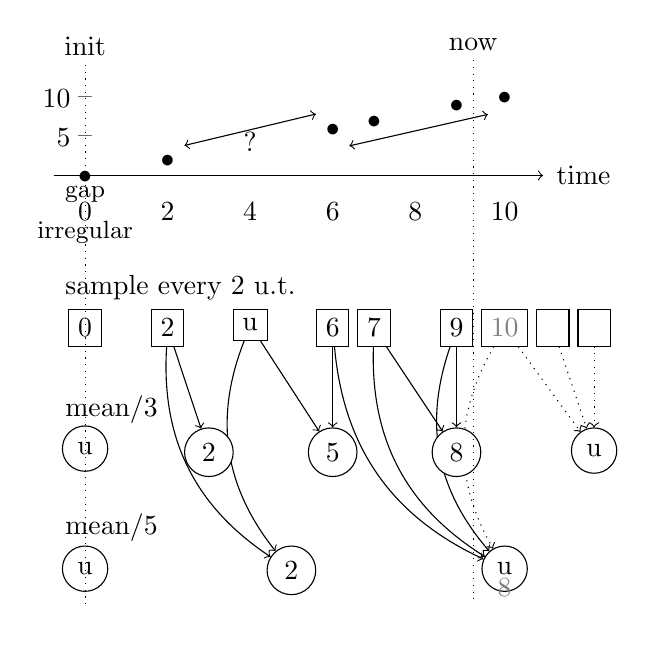
\begin{tikzpicture}

  \node[node distance=1mm] (0) {0};
  \node[node distance=1mm] (-1) [left=of 0]{\phantom{9}};
  \node[node distance=1mm] (1) [right=of 0] {\phantom{1}};
  \node[node distance=1mm] (2) [right=of 1] {2};
  \node[node distance=1mm] (3) [right=of 2] {\phantom{3}};
  \node[node distance=1mm] (4) [right=of 3] {4};
  \node[node distance=1mm] (5) [right=of 4] {\phantom{5}};
  \node[node distance=1mm] (6) [right=of 5] {6};
  \node[node distance=1mm] (7) [right=of 6] {\phantom{7}};
  \node[node distance=1mm] (8) [right=of 7] {8};
  \node[node distance=1mm] (9) [right=of 8] {\phantom{9}};
  \node[node distance=1mm] (10) [right=of 9] {10};
  \node[node distance=1mm] (11) [right=of 10] {\phantom{9}};
  \node[node distance=1mm] (12) [right=of 11] {\phantom{9}};


  \node [above=0 mm of 0] {$\bullet$}; 
  \node [above=2 mm of 2] (v2) {$\bullet$}; 
  \node [above=4 mm of 4] {?}; 
  \node [above=6 mm of 6] (v6) {$\bullet$}; 
  \node [above=7 mm of 7] {$\bullet$}; 
  \node [above=9 mm of 9] {$\bullet$}; 
  \node [above=10 mm of 10] (v10) {$\bullet$}; 


  \node[rectangle,draw] (s0) [below=of 0] {0};
  \node[rectangle,draw] (s2) [below=of 2] {2};
  \node[rectangle,draw] (s4) [below=of 4] {u};
  \node[rectangle,draw] (s6) [below=of 6] {6};
  \node[rectangle,draw] (s7) [below=of 7] {7};
  \node[rectangle,draw] (s9) [below=of 9] {9};
  \node[rectangle,draw] (s10) [below=of 10] {\color{gray}10};
  \node[rectangle,draw] (s11) [below=of 11] {\phantom{9}};
  \node[rectangle,draw] (s12) [below=of 12] {\phantom{9}};


  \draw[<->] (v2.north east) to (v6.north west)
  node [above,sloped,midway] {\small gap};

  \draw[<->] (v6.south east) to (v10.south west)
  node [below,sloped,midway] {\small irregular};

  
  %rd: 5s |inf| mean
  \node [circle,draw] (rd50) [below=4cm of 0] {u};
  \node [circle,draw] (rd55) [below=4cm of 5] {2};
  \node [circle,draw] (rd510) [below=4cm of 10] {u};
  \node [below=4.3cm of 10] {\color{gray}8};
 
  \draw[->,bend right] (s4) to (rd55);
  \draw[->,bend right] (s2) to (rd55);

  \draw[->,dotted,bend right] (s10) to (rd510);
  \draw[->,bend right] (s9) to (rd510);
  \draw[->,bend right] (s7) to (rd510);
  \draw[->,bend right] (s6) to (rd510);

  
  %rd: 3s |inf| mean
  \node [circle,draw] (rd30) [below=of s0] {u};
  \node [circle,draw,fill=white] (rd33) [below=2.5cm of 3] {2};
  \node [circle,draw,fill=white] (rd36) [below=2.5cm of 6] {5};
  \node [circle,draw,fill=white] (rd39) [below=2.5cm of 9] {8};
  \node [circle,draw] (rd312) [below=2.5cm of 12] {u};

  \draw[->] (s2) to (rd33);

  \draw[->] (s6) to (rd36);
  \draw[->] (s4) to (rd36);

  \draw[->] (s9) to (rd39);
  \draw[->] (s7) to (rd39);

  \draw[->,dotted] (s12) to (rd312);
  \draw[->,dotted] (s11) to (rd312);
  \draw[->,dotted] (s10) to (rd312);



  %eixos
  \node (et0) [above=1mm of -1] {};
  \node (et12) [above=1mm of 11] {};
  \node [right=-2mm of et12] {time};
  \draw[->] (et0) to (et12);
  \node (y5) [above=5mm of 0] {--};
  \node [left=-1.5mm of y5] {5};
  \node (y10) [above=10mm of 0] {--};
  \node [left=-1.5mm of y10] {10};

  \node (inici) [above=3.1cm of s0] {init};
  \node (inici2) [below=3.3cm of s0] {};
  \draw[-,dotted] (inici) to (inici2);

  \node (fi) [above=3.4cm of s9.east] {now};
  \node (fi2) [below=3.5cm of s9.east] {};
  \draw[-,dotted] (fi) to (fi2);


  % \node (fut) [below right=1mm and 1mm of fi] {future};
  % \draw[->] (fut.south west) to (fut.south east);

  % \node (pas) [below left=1mm and 1mm of fi] {past};
  % \draw[->] (pas.south east) to (pas.south west);

  \node [above=0cm of s0] {\makebox[0.5cm][l]{sample every 2 u.t.}};
  \node [below=0.5cm of s0] {\makebox[0.5cm][l]{mean/3}};
  \node [below=2cm of s0] {\makebox[0.5cm][l]{mean/5}};

\end{tikzpicture}



%%% Local Variables:
%%% TeX-master: "../main"
%%% ispell-local-dictionary: "british"
%%% End:

%   \caption{Multiresolution snapshot diagram with irregular sampling}
%   \label{fig:mtsms:sequence-irregular}
% \end{figure}



At the bottom of Figure~\ref{fig:mtsms:sequence} there is a diagram
showing the multiresolution action. The first row shows the numerical
time series' values corresponding to the above plot; the time series
is sampled every one unit of time. The second and the third row show a
particular schema of a multiresolution database consisting in two time
resolutions for the time series: one computes the mean of the sampled
values every three u.t.\ and the other computes the mean every five
u.t. In this example, computing the mean acts as selecting information
by aggregate statistics. All data stored before zero time is unknown
(\emph{u}) as has not been acquired. For the future values it is also
marked as \emph{u} until time advances.

The arrows of the figure show that every three sampled values a mean
is stored and, independently, every five values another mean is
stored. For the future values, dashed arrows show that if time
advances one u.t.\ then value 10 is sampled and the mean for time 10
can be computed resulting 8 but not yet the mean for time 12.

% Fig.~\ref{fig:mtsms:sequence-irregular} is essentially the same but
% showing two possible monitoring irregularities: a gap and a time
% disruption. In other words, we want to sample the time series every 2
% u.t.\ but first for some reason it can not be done in time 4 and
% second the sampling clock is disrupted and samples are done in time 7
% and 9 instead of 8. The resulting stored time schema is the same: on
% time resolution every 3 u.t.\ and the other every 5 u.t.; that is,
% without time disruptions. The resulting stored values are computed
% from the known sampled values, some coincide with
% fig.~\ref{fig:mtsms:sequence} whereas some differ specially in the
% gap. A better function than mean would solve this, we extend this
% further in section~\ref{sec:model:interpolador}.



%%% Local Variables:
%%% TeX-master: "main"
%%% ispell-local-dictionary: "british"
%%% End:

%  LocalWords:  multiresolution TSMS MTSMS


%model MTSMS

\section{Time series model}
\label{sec:model:TSMS}

Following current database models, a \acro{TSMS} model consists of two
components: a data model and a set of operations. \emph{Measures} and
\emph{time series} are the main objects of our \acro{TSMS} model.
%
In this section we describe and formalise the \acro{TSMS} model. 


\subsection{Data model}

Roughly speaking a \emph{time series} is a set of observations
collected at specific time instants. An observation may consist of
single value or multiple values collected at the same time instant.
Each pair of time and observed values is referred to as a
\emph{measure}. Then, a time series is a correspondence between times
and values. A time series can be described by a set of measures.

We name \emph{time domain} the set $\cal{T}$ of all the possible time
values. $\cal{T}$ can be either a finite or an infinite set and
usually it is a closed set. Although time is a complex issue
\cite{iep:time-supplement}, in this paper we will assume that the
$\cal{T}$ is the set of affinely extended real numbers $\Rb = \R \cup
\{+\infty,-\infty\}$. This avoids the complex details of time
modelling while being powerful enough for our purposes. Next, we
define the main time related concepts using this naive approximation.



\begin{definition}[Time concepts]
  \label{def:model:temps}
  Let $\cal{T}=\Rb$ be the domain for time.
  %
  We name an element $t\in\cal{T}$ as \emph{time instant}.
  %
  Let $s,t\in\cal{T}$ be two time instants.  We define the
  \emph{duration of time} between $s$ and $t$ as the value $d
  \in\cal{T}$ which measures the distance in time units between the
  two time instants, that is $d =|s-t|$.
\end{definition}

The \emph{value} is an attribute that indicates the magnitude of a
measure. The domain for the values can be any data type. Valid domains
for values include integers, real numbers, strings, and more
elaborated data structures such as arrays, lists, or even other time
series. Here below, the domain for values will be denoted by
$\cal{V}$. 
%
Without loss of generality in this paper we will assume that the
domain of values is the set of projectively extended reals $\Rp = \R
\cup \{\infty\}$.

A measure represents an actual value measured in a particular time
instant. We define it below.

\begin{definition}[Measure]
  Let $v\in\cal{V}$ be a value and let $t\in\cal{T}$ be the time
  instant when the value was acquired. We define a \emph{measure} $m$
  as the tuple $m=(t,v)$. The domain of a measure $m$, written as
  $\dom m$, is the domain of its value.
\end{definition}

Let $m = (t,v)$ be a measure. In what follows, $V(m)$ denotes the
value $v$ and $T(m)$ denotes the time $t$.

Order between measures plays an important role. Given two measures we
define two distinct \emph{order relations}.

\begin{definition}[Semitemporal order]\label{def:semitemporal_order}
  Let $m$ and $n$ be two measures. We name \emph{semitemporal order}
  the binary relation written $m\leq n$, defined as $m\leq n\iff
  (T(m)<T(n) \vee ( T(m)=T(n) \wedge V(m) = V(n) ))$.
\end{definition}

\begin{definition}[Temporal order]\label{def:temporal_order}
  Let $m$ and $n$ be two measures. We
    name \emph{temporal order} the binary relation written $m \leq^t
    n$ and defined as $m \leq^t n \iff T(m) \leq T(n)$.
\end{definition}

Note that the semitemporal order is a partial order while the temporal
order is a total order.

Intuitively speaking a \emph{time series} is a ordered set of measures of the
same phenomena.  Sometimes they are also called \emph{time
sequences}~\cite{last:hetland}. We define it as follows.

\begin{definition}[Time series]
  \label{def:model:timeseries}
  Let $S = \{m_0,\ldots,m_k\}\subset\cal{T}\times\cal{V}$ be a finite
  set of measures of the same type. Then, $S$ is a \emph{time series}
  iff $\forall i,j: i,j\in[0,k] \wedge i\neq j: T(m_i)\neq T(m_j)$.
  We define the domain of a time series $S$, denoted as $\dom S$, as
  the domain of its measures.
\end{definition}

Observe that although measures in $S$ are expected to be of the same
phenomena, from a formal standpoint we only require the domain of all
values to be the same. 

In a time series there are not two measures with the same time. Thus,
considering the temporal order, a time series is a totally ordered
set.

The \emph{cardinality} of a time series $S=\{m_0,\dots,m_k\}$, noted as
$|S|$, is the number of measures that contains.  An \emph{empty time series} is
noted as $\emptyset$. Needless to say, $|\emptyset|=0$.

Although we defined values as scalars, it is easy to extend the
concept. Following~\cite{assfalg08:thesis}, a time series can record
more than one phenomena if they share the same acquisition time
instants.  This kind of series are known as \emph{multivalued time
  series}. Let $S$ be a multivalued time series and let its domain be
$\dom S={\cal{V}}_1\times\cdots\times{\cal{V}}_n$. Then, we write its
measures as $m=(t,v_1,v_2,\ldots,v_n)$.



A time series is \emph{regular} when its measures are equi-spaced in time,
according to \cite{last:hetland}.  Let $S=\{m_0, m_1,\ldots,
m_{k-1},m_k\}$ be a time series, where
$T(m_0)<T(m_1)<\dots<T(m_{k-1})<T(m_k)$, and let $d\in\cal{T}$ be a
time duration. Then $S$ is \emph{regular} when $d=T(m_1)-T(m_0)=
\dots =T(m_k)-T(m_{k-1})$.




\subsection{Operations}
\label{sec:model:operations}

Time series can be manipulated through the operations defined in this
section.
%
Like the relational model operations, operations over time series
ignore the actual semantics of the data. In a particular application,
it should be decided whether an operation is semantically coherent or
must not be applied. For example, the addition of values coming from two
different phenomena could be semantically erroneous.

In this section three groups of operations are formalised, one in each
of the subsections which follow. The set operations, that consider
times series as sets; the sequence operations, that consider time
series as sequences; and the temporal operations, that manipulate the
time series assuming that are representations of functions.



\subsubsection{Set operations}
\label{sec:set}

We describe how common set operators can be applied to time series. We
rely on how the relational model of \acro{DBMS} describes operations
based on set algebra~\cite{date:introduction}.

Consider a time series $S$. $S$ is a finite ordered set (by the
temporal order). Then, if $S$ nonempty, $S$ has a maximum and a
minimum.  
%
The \emph{maximum}
of $S$, denoted as $\max S$, is an element of $S$ such that $\forall m
\in S:\max S\geq^t m $.  
%
Note that $\max S$ is not defined when $S=\emptyset$. However, the
time series has a supremum even when empty. In fact, according
to~\cite{cantrell:extendedreal}, $\sup \emptyset=-\infty$.
%
Let $m=(-\infty,\infty)$ be a measure with infinite time and value.
Using this fact we define the \emph{supremum} of $S$, noted as
$\sup S$, as
\[
\sup S =\begin{cases}
  \max S    & \text{when $S$ nonempty}\\
  m   & \text{otherwise}
\end{cases}
\]
Dually, we can define the \emph{minimum} of $S$, noted as $\min S$,
and the \emph{infimum} of $S$, noted as $\inf S$.

The \emph{membership} operation defines when a measure belongs to a time
series. We define two distinct membership operations which consider
the semitemporal order (Definition~\ref{def:semitemporal_order}) and
the temporal order (Definition~\ref{def:temporal_order}). In
consequence, they induce two different ways to consider time series
and its operations.

Let $S$ be a time series and $m$ be a measure. 
%
We say that $m$ belongs to $S$ (plain \emph{membership}), denoted as
$m \in S$, when $\exists x\in S: x=m$.  We also say that $m$ belongs
temporally to $S$ (\emph{temporal membership}), denoted as $m \inst
S$, when $\exists x\in S : T(m)=T(x)$.


The two distinct membership criteria induce two meanings for
inclusion. Let $R$ and $S$ be two time series.  We say that $R$ is
\emph{included} in $S$, written $R\subseteq S$, when all the elements
of $R$ belong to $S$.  Analogously, we say that $R$ is \emph{included
  temporally} in $S$, noted $R\subseteqt S$, when all the elements of
$R$ belong temporally to $S$.


The \emph{union} of two sets is a set containing elements from both
sets. Usual set union operations do not apply to time series because
the result time series could have repeated time values.  Thus, we 
give a slightly modified concept for union.

The union operation requires both time series to have the same domain,
as is also true with the union operation of relational
algebra~\cite{date:introduction}.

Let $R$ and $S$ be two time series and let $\dom R =\dom S$. 
%
The \emph{union} of $R$ and $S$, noted $R\cup S$, is a new time series
$R \cup S = \{m|m\in R\vee (m\in S\wedge m \notinst R)\}$. 
%
The \emph{temporal union} of $R$ and $S$, noted $S_1 \cupt S_2$, is a
time series $R \cupt S = \{ m | (m \in R \wedge m \in S) \vee (m \in R
\wedge m \notinst S) \vee (m \in S \wedge m \notinst R) \}$.  
%
It is interesting to emphasise that the union is a non commutative
operation while the temporal union is a commutative one.

\begin{figure}
  \centering
  %\def\escala{0.9}

\def\nodeA{node [above left=0.5cm and 0.1cm] {$(1,1)$} node [below left=0.5cm and 0.1cm] {$(5,1)$}}
\def\nodeB{node [above right=0.5cm and 0.1cm] {$(2,2)$} node [below right=0.5cm and 0.1cm] {$(6,2)$}}
\def\nodeT{node [above=0.1cm] {$(4,0)$} node [left=0.4cm] {$(3,1)$} node [right=0.4cm] {$(3,2)$}}
% Definition of circles
\def\firstcircle{(0,0) circle (1.5cm)}
\def\secondcircle{(0:2cm) circle (1.5cm)}
\def\thirdcircle{(0:1cm) circle (1.11cm)}

\colorlet{circle edge}{blue!50}
\colorlet{circle area}{blue!20}

\tikzset{
  filled/.style={fill=circle area, draw=circle edge, thick},
  outline/.style={draw=circle edge, thick},
  every node/.style={transform shape}
}

%\setlength{\parskip}{5mm}






%Set A or B
\begin{tikzpicture}[scale=\escala]
  \draw[filled] \firstcircle \nodeA;
    \begin{scope}
        \clip \secondcircle;
        \draw[filled, even odd rule] \firstcircle \nodeA
                                 \secondcircle 
                                 \thirdcircle;
   \end{scope}
    \draw[outline] \firstcircle
                   \secondcircle \nodeB
                   \thirdcircle \nodeT;

   \node[anchor=south] at (current bounding box.north) {$S_1 \cup S_2$};
\end{tikzpicture}
%Set temporal A or B
\begin{tikzpicture}[scale=\escala]
    \draw[filled, even odd rule] \firstcircle \nodeA
                                 \secondcircle \nodeB
                                 \thirdcircle \nodeT;
    \node[anchor=south] at (current bounding box.north) {$S_1 \cup^t S_2$};
\end{tikzpicture}






%%% Local Variables:
%%% TeX-master: "../main"
%%% ispell-local-dictionary: "british"
%%% End:

  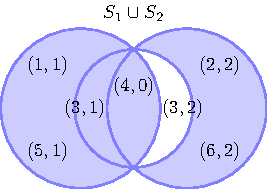
\includegraphics{fig_model_venn.pdf}
  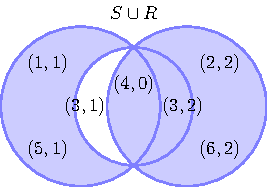
\includegraphics{fig_model_venn_reverse.pdf}
  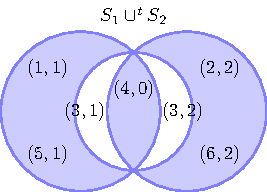
\includegraphics{fig_model_venn2.pdf}
  \caption{Venn diagrams for set and temporal set union operations of
    \acro{TSMS}}
  \label{fig:model:venn}
\end{figure}


\begin{example}\label{ex:model:s1s2}
  Let $R=\{(1,1), (3,1), (4,0), (5,1)\}$ and $S=\{(2,2), (3,2), (4,0),
  (6,2)\}$ be two time series. The union of $R$ and $S$ is $R\cup
  S=\{(1,1), (2,2), (3,1), (4,0), (5,1), (6,2)\}$. Because union is
  not symmetric, $S\cup R=\{(1,1), (2,2), \allowbreak(3,2), (4, 0), (5,1),
  (6,2)\}$. The temporal union results in $R\cupt S= S \cupt
  R=\{(1,1), (2,2), (4,0), (5,1), (6,2)\}$.  
  %
  Venn diagrams for all three cases are shown in
  Figure~\ref{fig:model:venn}, where the coloured area depicts the
  result time series. In every diagram, the central intersection area
  contains measures that share both time and value attributes, like
  instance $(4,0)$. The central left area contains the measures in $R$
  that only share the time attribute with a measure in $S$, like
  instance $(3,1)$. The central right area has a symmetrical
  meaning. The left and right outer areas are the remaining measures
  of $R$ and $S$ respectively.
\end{example}




Time series \emph{difference} can also be defined. Like union, the
difference requires both time series to have the same domain.
%
Let $R$ and $S$ be two time series and let $\dom R = \dom S$.
%
The \emph{difference} between $R$ and $S$, written $R-S$, is a time
series $R-S=\{m|m\in R\wedge m\notin S\}$.
%
The \emph{temporal difference} between $R$ and $S$, denoted $R-^t S$, 
is a time series $R-^t S=\{m|m\in R\wedge m \notinst S\}$.


Based on union and difference we can define \emph{intersection} as
$R\cap S = R - (R - S)$ and \emph{symmetric difference}
as $R \ominus S = (R - S) \cup (S - R)$. The
corresponding temporal operations can also be defined.


Relational \acro{DBMS} extend the set operators by some more such as
selection, rename or join. This kind of operators also make sense for
time series. To illustrate this possibility we define the join
operator.

Roughly speaking, the join of two time series is the combination of
measures sharing the same time attribute.  Let $R$ and $S$ be two time
series.  The \emph{join} of $R$ and $S$, denoted $R \join S$, is a
multivalued time series $R \join S = \{ (t,v_1,v_2) | (t,v_1) \in
R\wedge (t,v_2) \in S\}$. Note that $\dom(R\join
S)=\dom R\times\dom S$.
%
It must be noted that join requires both time series measures to share
exactly the same times. When time series diverge, the temporal
function operations explained later can be applied to adjust the time
instants to join requirements.


A \acro{DBMS} requires computational operators to provide opportunity
to calculate using the data contained. Relational \acro{DBMS} supply
operators like extend, aggregate or
summarise~\cite{date:introduction}. For time series, we define the more
general computational operators \emph{map} and \emph{fold}.

The map operator transforms a time series $S$ into a new time series
$R$ by applying a function to every measure.  Let $S$ and $R$ be two
time series, let $\cal{V}=\dom S$ and $\cal{V'}=\dom R$, and let
$f:\cal{T}\times\cal{V}\rightarrow\cal{T}\times\cal{V'}$ be a function
over a measure returning a measure. The \emph{map} of $f$ over $S$ is
a new time series defined as $\map(S,f)=\{f(m)|m\in S\}$. Note that
$\dom(\map(S,f))=\cal{V'}$.
%


The fold operator recursively combines every measure of a time
series. Assuming that $\mathcal{P}(C)$ is the powerset of $C$, we
define fold as follows.
%
Let $S=\{m_0,\dots, m_k\}$ and $R$ be two time series, let
$\mathcal{V}=\dom S$, let $\mathcal{V'}=\dom R$ and let 
%
$f:\mathcal{P}(\mathcal{T}\times\mathcal{V'}) \times (\mathcal{T}\times\mathcal{V}) \rightarrow \mathcal{P}(\mathcal{T}\times\mathcal{V'})$ 
%
be a function over a time series and a measure, which returns a time
series.
%
The \emph{fold} of $S$ by $f$ with initial value $R$ is a new time
series defined as $\fold(S,R,f) = f(\cdots(f(f(f(R,m_0),\allowbreak
m_1),\allowbreak m_2)\cdots),\allowbreak m_k)$.
%



The classical aggregation operator combines the data of a time series
into a single value.  It is worth to note that it is a special
case of fold.

Let $S=\{m_0,\dots,m_k\}$ be a time series, let $\mathcal{V}=\dom S$,
let $m$ be a measure with $\dom m=\mathcal{V}$, and let 
%
$f:(\mathcal{T}\times\mathcal{V})\times(\mathcal{T}\times\mathcal{V})\rightarrow \mathcal{T}\times\mathcal{V}$ 
%
be a function over two measures returning a measure. The
\emph{aggregate} of $S$ by $f$ with initial value $m$ is a new time
series defined as $\agg(S,m,f) = f(\cdots(f(f(f(m,m_0),\allowbreak
m_1),\allowbreak m_2)\cdots),\allowbreak m_k)$.  

% In the previous fold, the measures are computed in random order.
% However in some computational operations it is necessary to define the
% order, especially when $f$ is not commutative.  Then, it is possible
% to define a \emph{fold with order} as an extension of fold where
% measures are computed in a predetermined order.

% We define a
% \emph{fold with order}, $\orderfold$, as an extension of fold with a
% function $o$ that selects measures in order where $o: S_a \mapsto m_r$
% \[
%  \orderfold(S,S_i,f^f,o) =
%   \begin{cases}
%     S_i  \text{ if } |S|=0, \\
%     \orderfold(S_o,f^f(S_i,m_o),f^f,o)  \text{ else}
%   \end{cases}
% \]
% where $m_o = o(S)$ and $S_o = S - \{m_o\}$.



\begin{example}
\label{ex:computational-operators}
Let $S=\{(1,1),(2,3),(4,1)\}$ be a time series.  Map operator allows
computing a new time series whose values result from time multiplied
by value.  We define the map function $f(t,v)=(t,t\cdot v)$. Then
$\map(S,f)=\{(1,1),(2,6),(4,4)\}$.  
%


The aggregate operator allows, for instance, to compute the measure
that results from the sum of all the values.  To illustrate it, we
define the aggregate function $f(m,n)=(0,V(m)+V(n))$. Now,
$\agg(S,(0,0),f) = (0,5)$, where $5$ is the sum of all the values of
$S$. Note that time is meaningless in this computation.

The fold operator allows, for instance, to select the measures having
its value equal to one.  We define the fold function $f(R,m)=R\cup R'$
where $R'=\{m\}$ if $V(m)=1$ or $R'=\emptyset$ otherwise. Let $m$ be
any measure, note that $f(\emptyset,m)= R'$. Then
$\fold(S,\emptyset,f)=\{(1,1),(4,1)\}$.
\end{example}

%%%%%%% BINARY COMPUTATIONAL OPERATORS

Finally we describe how, using the operators defined before, we can
implement \emph{binary computational} operators between two time
series. This illustrates the power of the operators defined so far.
%

The strategy requires first to join the two time series and then
apply the computational operations. 
%
Let $S$ and $R$ be two time series and $\odot$ be a binary operator on
the value domain. The operator $\odot$ can be extended to the time
series as:
%
$S\odot R=\map(S\join R, f)$ being $f$ the function
$f(t,v,w)=(t,v\odot w)$.
%
This allows to extend real binary operations such as sum, $R+S$, or
division, $R/S$, to time series.


\subsubsection{Sequence operations}
\label{sec:sequence}

Sequence operations manipulate time series considering measures as
being totally ordered by time.  We define three basic operations:
\emph{slice}, \emph{successor} and \emph{concatenation}.


The classical interval concept can be applied to time domain. In this
context, given two time instants $s$ and $t$, we use the notation
$[s:t]$, $(s:t)$, $[s:t)$ and $(s:t]$ respectively for the closed
interval, open interval, open right and open left interval.
%
Following~\cite{last:hetland}, to slice a time series $S$ means to
extract a new time series $R\subseteq S$ constrained to a given time
interval. We denote this operation as the original time series followed
by the interval. Therefore, $S[s:t]=\{m|m\in S \wedge
T(m)\in[s:t]\}$. We can use other intervals to slice a time series in
a same fashion. For instance, $S(s:t]=\{m|m\in S \wedge
T(m)\in(s:t]\}$.

The ordinary time order allows to define the concepts of successor and
predecessor for the measures of a time series.
%
Let $S=\{m_0,\ldots,m_k\}$ be a time series and $m$ be an arbitrary
measure.
%
We say that $m_i=\nex_S(m)$ is the \emph{next} measure to $m$ in $S$ if and
only if $m_i=\inf(S(T(m):+\infty])$.  
%
We also say that $m_i=\prev_S(m)$ is the \emph{previous} measure to
$m$ in $S$ if and only if $m_i=\sup(S[-\infty:T(m)))$. 
%
Infinite measures are obtained when next and previous are applied to
supremum and infimum measures respectively: $\nex_S(\sup
S)=(+\infty,\infty)$ and $\prev_S(\inf S)=(-\infty,\infty)$.

To concatenate two time series means to compute a new time series with
the measures of the first time series followed in time order by the
measures of the second one. 
%
The concatenation requires both time series to share the same domain.
Let $R$ and $S$ be two time series and let $\dom R=\dom S$. The
\emph{concatenation} of $R$ and $S$, denoted as $R||S$, is a time
series that contains all the measures of $R$ together with those of
$S$ that do not intersect with the time interval of $R$. That is,
$R||S= R\cup (S - S[T(\inf R):T(\sup R)])$.



\subsubsection{Temporal function operations}
\label{sec:model:tfunc}

A time series can be thought as discrete representation of an
(original) temporal function. In this section we devise some
operations that manage the time series according to this temporal
function standpoint.  
%

The graph of a function allows to obtain and interpret the
continuous nature of a time series, when the domain of time and value
attributes can be plotted then the graph is equivalent to a graphical
representation.  
%
Let $S$ be a time series and $\cal{T}$ the time domain. The \emph{graph} of
the time series $S$ is a set of ordered pairs $\graph S
=\{(t,S(t))|t\in \cal{T}\}$ where $S(t)$ is a \emph{temporal representation
function} for the time series.
%


Given a time series $S$, the \emph{temporal representation function}
$S(t)$ is a function along the variable $t$ in the domain of
time and the target in the domain of values.
%
In some sense, $S(t)$ can be thought as the original temporal function
from which $S$ was obtained.
%

There is not an unique way to obtain $S(t)$ for a given time series
$S$. Because of this, in temporal representation functions we will
introduce a superscript, say $r$, that shows the name $r$ of the
representation method used. Then, $S(t)^r$ means the representation
function of $S$ using method $r$. Below, we exemplify the
representation functions using two different methods based on impulse
and constant piecewise functions.


\begin{definition}[Dirac representation] 
  Dirac delta (\dd) is a method of representation based on the Dirac
  delta function. Let $S$ be a time series. We define $S(t)^\dd$ as
  the following \dd{} representation function:
  \[
  S(t)^\dd
  =  \begin{cases}
          V(m) & \text{if } \exists m\in S:t=T(m) \\
          0    & \text{otherwise}
  \end{cases}
  \]
\end{definition}

\begin{definition}[Zohe representation]
  Zero-order hold everted (\zohe{}) is a method of representation
  based on the \emph{zero-order hold} signal reconstruction method. It
  is a piecewise constant function built from left-continuous step
  functions.  Let $S$ be a time series. We define $S(t)^\zohe$ as the
  following representation function:
  \[
  S(t)^\zohe 
  = \begin{cases}
    V(m) & \text{if } \exists m\in S: t\in \big(T(\prev_S(m)):T(m)\big]\\
    0    & \text{if } t > T(\max(S)) 
  \end{cases}
  \]
\end{definition}




The concept of representation is used for formalising some set and
sequence operators as temporal operators. 

% Consequently, the result of each one will depend on a representation
% method, which is indicated as a parameter.


We define a temporal interval operation to introduce this concept.
Let $S$ be a time series, let $[s:t]$ be an interval of two time
instants and let $r$ be a representation method. The \emph{temporal
  interval}, denoted as $S[s:t]^r$, returns a new time series with
measures in the interval temporal range. That is, $S[s:t]^r = S(u)^r$
for all $u \in [s:t]$. This is a general definition difficult to
implement, so for every representation a particular temporal interval
must be interpreted:

\begin{itemize}
\item Let $S(t)^\dd$ be the \dd{} representation for $S$. The
  \emph{\dd{} temporal interval} is $S[s:t]^\dd = S[s:t]
  \cup \{m\} \cup \{n\}$ where $m=(s,0)$ and $n=(t,0)$.

\item Let $S(t)^\zohe{}$ be the \zohe{} representation for $S$. The
  \emph{\zohe{} temporal interval} is $S[s:t]^\zohe{} = S(s:t]
  \cup \{m\}$ where $m=(t,v)$ and $v= V(\inf( S[t:+\infty] ))$.
\end{itemize}



From temporal interval other operators can be defined such as temporal
selection, temporal concatenation, or temporal join. As example the
definition of temporal interval operation is given.


The temporal selection over a time series allows to change the
resolution in the context of a representation function.  Let $S$ be a
time series, let $T=\{t_0,t_1,\dotsc,t_k\}$ be a set of time instants, and let 
$r$ be a representation method. The \emph{temporal selection}, denoted as
$S[T]^r$, is a time series with measures in $T$ times computed in
coherence with the representation method $r$. That is, $S[T]^r = S[t_0:t_0]^r
\cup S[t_1:t_1]^r \cup \dotsb \cup S[t_k:t_k]^r$. Let $t$ be a time
instant, note that temporal selection depends on the temporal interval
operation $S[t:t]^r$, which is equivalent to the notion of
temporal representation function over a single time instant. That is, $S[t:t]^r
= \{ (t, S(t)^r) \}$.




The temporal selection operation also allows to regularise a irregular
time series. Let $S$ be a time series, let $d,e\in\cal{T}$ be the
desired regularity parameters, and let $k\in\N$ be a limit for the
scope of the range.  A regularised $S$ can be obtained with $S[T]^r$
where $T = \{e+nd | n\in\N \wedge n\leq k \}$ is a set of time
instants equi-spaced.






\section{Multiresolution model}
\label{sec:MTSMS}

In this section we formalise a model for \acro{MTSMS}. Illustration
examples of the definitions given can be found at the end of the
section. Furthermore, in Section~\ref{sec:features} we have
intuitively introduced the concept of multiresolution through an
example.

A \acro{MTSMS} is a \acro{TSMS} that stores time series using a lossy
compression approach. 
%
The \acro{MTSMS} model is based on the concepts of \emph{measures} and
\emph{time series} as defined in Section~\ref{sec:model:TSMS}. We call
\emph{multiresolution time series} to each time series stored in a
\acro{MTSDB}.
%
A multiresolution time series is a collection of \emph{resolution
  subseries} that store a view of the original time series in a given
resolution.
%
The operator that adds data to a resolution subseries requires to
temporarily accumulate measures in a \emph{buffer}. This allow to
aggregate original data to obtain the expected resolution and finally
store them in a \emph{disc}.


\begin{figure}
  \centering
  %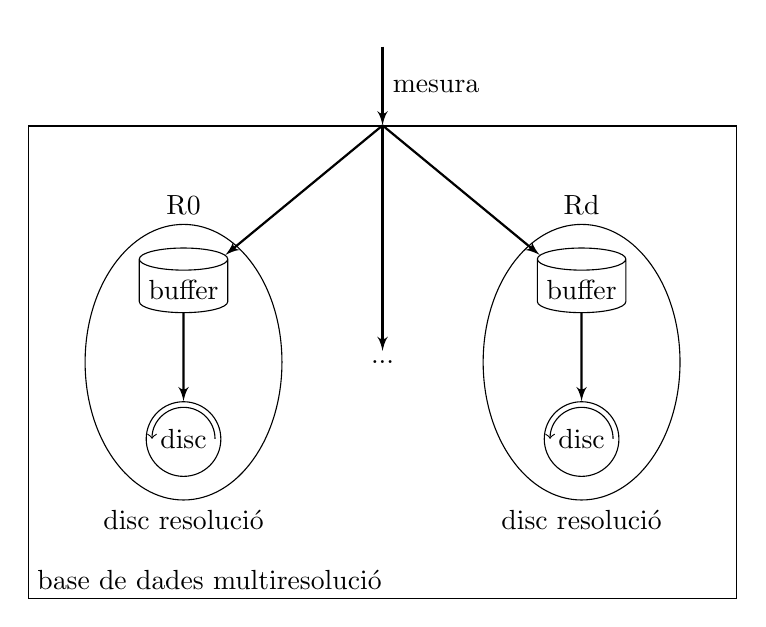
\begin{tikzpicture}
 \tikzset{
        myarrow/.style={->, >=latex',  thick},
      }
      

  \node[rectangle,draw,minimum height=6cm,minimum width=9cm] (m) {};
  \draw[shift=( m.south west)]   
  node[above right] {base de dades multiresolució};


  %discmig
  \node (m.center) (discr1) {...};

  %discr
  
  \node[ellipse,draw,minimum height=3.5cm,minimum width=2.5cm,alias=discr0] [left=of discr1] {};
  \node[above=0cm of discr0.north] {R0};
  \node[below=0cm of discr0] {disc resolució};

  \node[cylinder, draw, shape border rotate=90, aspect=0.25,alias=buffer0] [below=3mm of discr0.north] {buffer};
  \node[circle, draw,alias=disc0]  [above=3mm of discr0.south] {disc} ;
  \draw [->] (disc0.center)++(.4:.4cm) arc(0:180:.4cm);
  \draw[myarrow] (buffer0.bottom) -- (disc0.north);


  %discrd

  \node[ellipse,draw,minimum height=3.5cm,minimum width=2.5cm,alias=discrd] [right=of discr1] {};
  \node[above=0cm of discrd] {Rd};
  \node[below=0cm of discrd] {disc resolució};

  \node[cylinder, draw, shape border rotate=90, aspect=0.25,alias=bufferd] [below=3mm of discrd.north] {buffer};
  \node[circle, draw,alias=discd]  [above=3mm of discrd.south] {disc} ;
  \draw [->] (discd.center)++(.4:.4cm) arc(0:180:.4cm);
  \draw[myarrow] (bufferd.bottom) -- (discd.north);



  %mesura 
  \node[above=1cm of m.north] (m0) {};

  \draw[myarrow] (m0) -- (m.north) 
  node[right,midway] {mesura};

  \draw[myarrow] (m.north) -- (buffer0);
  \draw[myarrow] (m.north) -- (bufferd);
  \draw[myarrow] (m.north) -- (discr1);

\end{tikzpicture}
  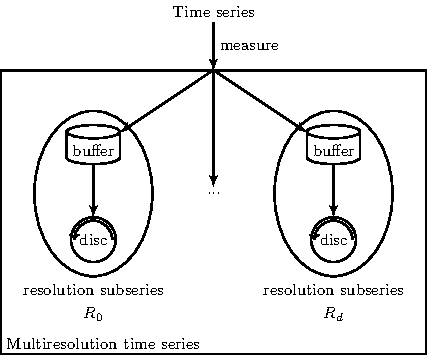
\includegraphics{fig_model_mtsdb.pdf}
  \caption{Architecture of \acro{MTSMS} model}
  \label{fig:model:mtsdb}
\end{figure}

Figure~\ref{fig:model:mtsdb} shows the architecture of a
\acro{MTSMS} for a single multiresolution time series.
%
In this way, the original time series gets stored in the resolution
subseries, each with a different time resolution and distinct
attribute aggregation policies. Discs are size bounded so they only
contain a fixed amount of measures. When a disc becomes full it
discards a measure. Thus, a multiresolution database is bounded in
size and the time series gets stored in a number of storage bounded
time subseries.

Regarding operations, the \acro{MTSMS} model requires two kind of
operators. Some operators should be devoted to set up the time
intervals between measures and to aggregate the attributes. Some other
operators should be dedicated to query the multiresolution schema and
to extract the time series data.

Following, we define the \acro{MTSMS} model structure and the
structural operators, the operations to query a multiresolution
schema, and the \emph{attribute aggregate functions}.  Although schema
manipulation operations could be defined, in this paper we exclusively
focus on structure and data query operators.


\subsection{Structure}

A \emph{buffer} is a container for a time series. The aim of the
buffer is to regularise the time series using a constant
\emph{resolution step} and an \emph{attribute aggregate function}.  We
name \emph{consolidation} to this action of regularisation.  Note that
the attribute aggregate functions are defined in
Section~\ref{sec:model:interpolador}.

\begin{definition}[Buffer]
  Let $S$ be a time series, let $\tau\in\cal{T}$ be the last
  consolidation time, let $\delta\in\cal{T}$ be the resolution step
  and let $f$ be an attribute aggregate function. We define a
  \emph{buffer} $B$ as the tuple $B=(S,\tau,\delta,f)$.
\end{definition}

An empty buffer is noted as $(\emptyset, t_0, \delta, f)$, that is an
empty time series, an initial consolidation time $t_0\in\cal{T}$, a
resolution step $\delta$ and a function $f$.  Given a buffer all the
consolidation time instants can be determined as $\tau_n=t_0+n\delta$
for all $n\in\N$.

Let $B=(S, \tau, \delta, f)$ be a buffer. The \emph{consolidation} of
$B$ is an operation that computes a new measure $m=f(S, \tau, \delta)$
summarising the data of $S$ comprised in the given interval.

A buffer has two main structural operations. The first one adds a
measure to the buffer and the second one consolidates the buffer.

Let $B=(S,\tau,\delta,f)$ be a buffer and let $m$ be a measure.  The
addition of $m$ to $B$, noted as $\addB(B,m)$, returns a new buffer
$\addB(B,m)=(S',\tau,\delta,f)$ where $S' = S \cup \{m\}$.

Let $B=(S,\tau,\delta,f)$ be a buffer. The consolidation of $B$, noted
as $\consB(B)$, returns a new buffer and a new measure $\consB(B)=(B',m')$
where $ B'= (S[\tau+\delta:+\infty], \tau+\delta,\delta,f)$ and $m' =
f(S,\tau,\delta)$. Note that after the consolidation, the
consolidated part of the time series can be removed from the buffer:
historic data is discarded.

The consolidation of a buffer is applied to the first non consolidated
time instant and the total consolidation is obtained by successive
application of the operator. 
%
This requires measures to be added by time order and to consolidate
the buffer when the time of some measure is bigger than the buffer's
next consolidation time.  
%
Let $B=(S,\tau,\delta,f)$ be a buffer and $m=\sup S$ the maximum
measure of $B$. We say that $B$ is consolidable if and only if $T(m)
\geq \tau+\delta$.

A \emph{disc} is a finite capacity container of measures. A time
series stored in a disc has its cardinal bounded. When the cardinal of
the time series is to overcome the limit, some measures need to be
discarded.

\begin{definition}[Disc]
  Let $k\in\N$ and $S$, $|S|\leq k$, be a time series. We define a
  \emph{disc} $D$ as the tuple $D=(S,k)$.
\end{definition}

An empty disc is noted as $(\emptyset,k)$. It is the tuple of an
empty time series and a bound $k$.

The main operation on a disc is to add a measure while keeping under
control the cardinal of the times series. Let $D=(S,k)$ be a disc and
let $m$ be a measure.  The addition of $m$ to $D$, written as
$\addD(D,m)$, is a new disc $\addD(D,m)=(S',k)$ where
%
\[
S' = \begin{cases}
  S\cup\{m\}                 & \text{if } |S|<k  \\
  (S-\{\min S\}) \cup \{m\} & \text{otherwise}
\end{cases}  
\]

A \emph{resolution subseries} is a structure that regularises and
aggregates a time series. It is composed of a buffer, which contains
the time series to be regularised, and a disc, which contains
the regularised time series.


\begin{definition}[Resolution subseries]
  Let $B$ be a buffer and let $D$ be a disc.  We define a
  \emph{resolution subseries} $R$ as the tuple $R=(B,D)$.  
\end{definition}
 
The operators of a resolution subseries extend the buffer and disc
ones. Let $R=(B,D)$ be a resolution subseries and let $m$ be new a
measure.  The addition of $m$ to $R$, noted as $\addR(R,m)$, is a new
resolution subseries $\addR(R,m)=(B',D)$ where $B'= \addB(B,m)$ is the
addition of the measure to the buffer.  The consolidation of $R$,
noted as $\consR(R)$, is a new resolution subseries
$\consR(R)=(B',D')$ where $(B',m') = \consB(B)$ is the consolidation
of the buffer and $D'= \addD(D,m')$ is the addition of the
consolidated measure to the disc. A resolution subseries is
consolidable only when its buffer is consolidable.

A \emph{multiresolution time series} is a set of resolution subseries
referred to the same time series. We store a time series regularised
with distinct resolutions across the resolution subseries, as
previously shown in Figure~\ref{fig:model:mtsdb}.

\begin{definition}[Multiresolution time series]
  Let $M=\{R_0, \dots, R_k\}$ be a finite set of resolution
  subseries. Then $M$ is a \emph{multiresolution time series}.
\end{definition}

Therefore, to define a multiresolution time series we must define the
number of resolution subseries and its corresponding parameters
$(\delta,\tau,f,k)$.  Usually there are no repeated pairs of
$(\delta,f)$ parameters among a multiresolution series, so they act as
key attributes.

The operators of a multiresolution time series apply to every
resolution subseries contained. Let $M=\{R_0,\allowbreak
\dots,\allowbreak R_k\}$ be a multiresolution time series and let $m$
be a measure.
%
The addition of a measure to every resolution subseries, noted as
$\addM(M,m)$, is a new multiresolution time series $\addM(M,m)=\{R'_0,
\dots,\allowbreak R'_k\}$ where $R'_i=\addR(R_i,m)$. The consolidation
of all resolution subseries, noted as $\consM(M)$ is a new
multiresolution time series $\consM(M)=\{R'_0,\allowbreak
\dots,\allowbreak R'_k\}$ where
\[R'_i=
\begin{cases}
\consR(R_i) & \text{if } R_i \text{ consolidable}\\
 R_i & \text{otherwise}
\end{cases}
\]

% The multiresolution consolidation operation should be applied
% regularly based on a consolidation clock. When the measure ordered
% addition approach is taken as explained in the buffer's consolidation,
% then there is no need for a clock in a \acro{MTSMS}. The consolidation
% clock is induced by the measure's addition and then it is only
% necessary to check the multiresolution consolidation operation on new
% additions. However, there could be other approaches where the
% consolidation clock was given by an external clock or external
% events. Then the consolidable definitions would depend on this
% external clock.





\subsection{Queries}

There are two basic time series queries for a \acro{MTSMS}: (i) to
extract a time subseries from a resolution subseries or (ii) to query
for a total time series from all consolidated data.

% Aquesta sembla una consulta una mica circumstancial i menor ...
Let $M$ be a multiresolution time series and let $(\delta,f)$ be a
pair of key attributes.  The first query, denoted as
$\seriedisc(M,\delta,f)$, is a time series such that $\exists (B,D)
\in M: B=(S,\tau,\delta,f) \wedge D=(\seriedisc(M,\delta,f), k) $
where $S,\tau,k$ are bound variables.  Note that we
assume there are no repeated $(\delta,f)$ pairs in $M$.

Let $M=\{R_0,\dots,R_k\}$ be a multiresolution time series and let
$S_0,\dots,S_k$ the time series corresponding to the resolution
subseries $R_0,\dots,R_k$. Assume that the attribute aggregation
functions of all $R_i$ are the same and the resolution steps of all
$R_i$ are distinct.
%
We note as $\totalseries(M)$, the time ordered concatenation of all
time subseries. Recall that $R||S$ is the concatenation for two time
series $R$ and $S$, which has been defined in
Section~\ref{sec:sequence}. Assume that $i_0,\dots,i_k$ is a
permutation of $[0,k]$ such that $\delta_{i_0} < \delta_{i_1} < \cdots
< \delta_{i_k}$ being $\delta_i$ the resolution step of the resolution
subseries $R_i$. Then, $\totalseries(M) = S_{i_0} || S_{i_1} || \cdots
|| S_{i_k}$.
%
TotalSeries obtains the better possible resolution.

From these aforementioned basic time series queries, more elaborated
queries can be applied to \acro{MTSMS} by using \acro{TSMS}
operations. For example, let $L$ and $M$ be two multiresolution time
series, we can compute the sum of both as $\totalseries(L) +
\totalseries(M)$. Recall that $R+S$ is the sum of the values of two
time series $R$ and $S$, which has been defined in
Section~\ref{sec:set} as a binary computational operator.


\subsection{Attribute aggregate function}
\label{sec:model:interpolador}

Attribute aggregate functions are a specific case of \acro{TSMS}
aggregate operations used to summarise time series data while
consolidating a buffer.
%
% Let $S$ be a time series and let $[x,v]$ be a
% time interval. An attribute aggregate function $f$ calculates a new
% measure $m=f(S,[x,v])$. Then, this resulting measure $m$ is interpreted to
% summarise the measures of $S$ for the consolidation interval $[x,v]$.

Let $S$ be a time series, let $\delta$ be a resolution step and let
$\tau$ be a consolidation time.  An \emph{attribute aggregate function} $f$
calculates a new measure $m=f(S,\tau,\delta)$. From $\tau$ and
$\delta$, we obtain the time interval $[\tau:\tau+\delta]$.  Then, the
resulting measure $m$ is interpreted to summarise the measures of $S$
for the time interval $[\tau:\tau+\delta]$.



% \[
% f : S=\{m_0,\ldots,m_k\} \times I=[t_i,t_j] \mapsto m'
% \]
% \[
% f: \cal{P}(\cal{T}\times\cal{V}) \times (\cal{T}\times\cal{T}) \rightarrow \cal{T}\times\cal{V}
% \]

An attribute aggregation function follows this general schema. First,
it obtains a time subseries $S'$ according to the consolidating
interval using a slice operator. For example, $S' =
S[\tau:\tau+\delta]$. Second, it applies a \acro{TSMS} aggregation
function on this time subseries to obtain $m$. For instance, $m =
\agg(S',n, f)$, being $f$ an aggregation function and $n$ an initial
measure, as defined in Section~\ref{sec:set}.

Many different attribute aggregate functions can be used in order to
summarise a time series, for example it is possible to calculate an
statistic indicator of the time series such as the average or a more
complex digital signal processing operation as proposed
by~\cite{zhang11}. Furthermore, the representation of a time series
and some of its pathologies can be considered during the aggregation
process.

Given the diversity of attribute aggregate functions, no global
assumptions can be made about them. Each user should decide which
combination of aggregation and representation fits better to the
measured phenomena.  Therefore, the \acro{MTSMS} model must have a
generic design that allows the users to define their own aggregate
functions.

In what follows we will give some examples of usual attribute
aggregation functions. These functions compute a new measure given a
set of known measures. Then, an attribute aggregation function should
compute a new \emph{time} and a new \emph{value} from the set known measures.
%
% For the rest of this Section we will write $m=f(S,[x,v])$ be the
% resulting measure of an attribute aggregation function $f$ applied to
% a time series $S$ for a time interval $[x,v]$.

% Sobre el calcul del nou temps

The attribute aggregation functions generally return measures that
match the buffer consolidating times. Assume, for instance, that $f$
is an attribute aggregation function and let $m=f(S,\tau,\delta)$.
Then, the time of $m$ is usually computed as $T(m)=\tau+\delta$.
%
However, in some cases it is preferred that $T(m)$ do not match the
buffer consolidating times.
%
For instance, the resulting measure can be aggregated from a time
subseries $S'$ using an open interval $S'=S(\tau:\tau+\delta)$, a
closed interval $S'=S[\tau:\tau+\delta]$, or other combinations like
$S'=S(\tau-d:\tau+\delta-d]$, where $d$ is a time duration that delays the
consolidation to $T(m)=\tau+\delta-d$.
%
This time offset can also be variable. For example, an aggregate
function that returns the first measure of the interval
$m=\min(S[\tau:\tau+\delta))$, then the resulting time fulfils that
$\tau\leq T(m) < \tau+\delta$.

% Sobre el calcul del nou valor
Assume that $f$ is an attribute aggregation function and let
$m=f(S,\tau,\delta)$.  An attribute aggregation function $f$ should
compute the value of $m$.
%
Next there are some examples that illustrate how to compute $V(m)$
based on the temporal function time series operators. 
That is, the time series aggregated is interpreted by the temporal
representation function $S(t)^r$ as has been described in
Section~\ref{sec:model:tfunc}. 
%
In these example functions we leave the time series representation $r$
uninstantiated.

\begin{itemize}
\item The \emph{maximum} computes $V(m)$ as $V(m) =
  \max\limits_{\forall t \in [\tau:\tau+\delta]} S(t)^r$. It
  summarises $S$ with the maximum of the measure values in the
  interval $[\tau:\tau+\delta]$.
\item The \emph{last} computes $V(m)$ as $V(m) = S(\tau+\delta)^r$. It
  summarises $S$ with the value at $\tau+\delta$ time instant.
\item The \emph{mean} computes $V(m)$ as $V(m) = \frac{1}{\delta}
  \int\limits_{\tau}^{\tau+\delta} S(t)^r dt$. It summarises $S$ with
  the mean of the function in the interval $[\tau:\tau+\delta]$.
\end{itemize}

The time series representation in previous examples can be
instantiated in several ways. In what follows we exemplify this
instantiating $r$ as \dd{} and \zohe{}.

Dirac delta attribute aggregation functions interpret the resulting
time as centered on the interval $T(m)=\frac{2\tau+\delta}{2}$. The
resulting value $V(m)$ depends on the attribute, let
$S'=S[\tau:\tau+\delta]^\dd$ be the selection of measures by Dirac
delta temporal interval. Then,
\begin{itemize}
\item The $maximum^\dd$ is such that $V(m) =
  \max\big(0,\max\limits_{\forall n \in S'} V(n)\big)$.
\item The $last^\dd$ is such that $V(m) = V(\max S')$.
\item The $mean^\dd$ is such that $V(m) = \frac{1}{\delta}
  \sum\limits_{\forall n \in S'} V(n)$. Note that for the Dirac
  delta function $\int\dd(t)dt=1$.
\end{itemize}

Note that $\sum\limits_{\forall n \in S'} V(n)$ is a sum of values
that could be implemented as $\agg(S',(0,0),f)$ where
$f(m,n)=(0,V(m)+V(n))$, as shown in
Example~\ref{ex:computational-operators}.

\zohe{} attribute aggregation functions interpret the resulting time
as the right limit of the interval $T(m)=\tau+\delta$. The resulting
value $V(m)$ depends on the attribute, let
$S'=S[\tau:\tau+\delta]^\zohe{}$ be the selection of measures by
\zohe{} temporal interval. Then,

\begin{itemize}
\item The $\maxz$ is such that $V(m) = \max\limits_{\forall n \in S'}
  V(n)$.
\item The $last^\zohe{}$ is such that $V(m) = V(\max S')$.
\item The $\meanz$ is such that $V(m) = \frac{1}{\delta}
  \big[(T(o)-\tau)V(o) + \sum\limits_{\forall n\in R}( T(n)-
  T(\prev_S n) )V(n)\big]$ where $o=\min S'$ and $R= S' - \{o\}$.
\end{itemize}

Note that  $\meanz$ is a sum of values
that could be implemented as $\meanz = \frac{1}{\delta}\agg(S',(0,0),f)$ where $f(m,n)=(0,V(m)+v)$ and 
\[
 v= 
 \begin{cases}
   (T(n)-\tau)V(n) & \text{if } n=\min S'\\
   (T(n)-T(\prev_{S'} n))V(n) & \text{else }
 \end{cases}
\]

\emph{RRDtool}, \cite{rrdtool}, uses an aggregation function similar
to $\meanz$ to summarise velocity counter data by keeping the area
below the original signal.

It is interesting to note that some attribute aggregation patterns are
very similar. For instance, the maximum and last attribute aggregation
schemes differ basically on the interval selection operation. However,
other patterns have a more elaborated interpretation depending on the
actual representation used. This is the case of $\meanz$ and $mean^\dd$.


\begin{example}\label{ex:model:smultiresolution} 
  We define a multiresolution schema for a time series, we consolidate
  the database and we query its data.  Let $S = \{
  (1,6),(5,2),\allowbreak (8,5),\allowbreak (10,0),\allowbreak
  (14,1),\allowbreak (19,6),\allowbreak (22,11),\allowbreak
  (26,6),(29,0) \}$ be a time series and let $M=\{R_0,R_1\}$ be a
  multiresolution time series where each resolution parameters are
  $\tau_0=0$ , $\delta_0=5$, $f_0 =\meanz$, $k_0=4$ and $\tau_1=0$,
  $\delta_1=10$, $f_1 =\maxz$, $k_1=2$. Therefore $R_0$ will be
  consolidated at time instants 5, 10, 15, 20, 25, 30\dots and $R_1$
  at 10, 20, 30\dots

  All measures of $S$ are added to $M$
  and then it is consolidated until it is no more consolidable. As
  $T(\max S)=29$, the last consolidation times are $\tau_0=25$ and
  $\tau_1=20$, so we call $M_{29}$ to the multiresolution time series
  at this state.

  Then, the two time subseries consolidated are obtained by querying
  $\seriedisc(M_{29},5,\allowbreak \meanz)=\{\allowbreak
  (10,3),\allowbreak (15,\allowbreak 2),\allowbreak (20,7),\allowbreak
  (25,8)\}$ and $\seriedisc(M_{29},\allowbreak 10,\allowbreak \maxz)
  =\allowbreak \{ \allowbreak (10,6),\allowbreak (20,11)\}$. Regarding
  buffers, let $S_0$ and $S_1$ be the $M_{29}$ buffer's time series,
  note that $S_0= \{\allowbreak (26,6),\allowbreak (29,0)\allowbreak
  \}$ and $S_1=\{\allowbreak (22,11),\allowbreak (26,6),(29,0)\}$.

  In this particular example,
  $ \totalseries(M_{29}) = \seriedisc(M_{29},\allowbreak 5,\meanz)$ as $R_0$ has
  twice the resolution than $R_1$ and $k_0$ is bigger than $k_1$. 
\end{example}



%%% Local Variables:
%%% TeX-master: "main"
%%% ispell-local-dictionary: "british"
%%% End:

% LocalWords:  genericity multiresolution subseries consolidable

% LocalWords:  pathologies MTSMS TSMS cardinality multivalued infimum
% LocalWords:  multivalues supremum tuple affinely projectively MTSDB
%  LocalWords:  semitemporal piecewise TotalSeries RRDtool


%exemple



\section{Example}
\label{sec:example}


Next we show a real example database for a time series data. Actual
data comes from a temperature distributed sensor monitoring system
\cite{alippi10}, we focus on one sensor data. We use Pytsms and
RoundRobinson implementations in order to create a \acro{MTSDB} and
to query it.

\emph{Data}. The Figure~\ref{fig:exemple:original} shows the original
data for one year and a half. The plot interpolates linearly the
measures. In this plot we can see that there is missing data and some
outlying observations. There are $146\,709$ stored values.

\begin{figure}[tp]
  \centering
  %\tikzset{every picture/.style={scale=0.8}}
  %\tikzsetnextfilename{fig_exemple_original}
  %\usetikzlibrary{dateplot}    
\begin{tikzpicture}
    \begin{axis}[
        date coordinates in=x,
%        xticklabel={\pgfcalendar{tickcal}{\tick}{\tick}{\pgfcalendarshorthand{m}{.}}},
        xticklabel={\pgfcalendarmonthshortname{\month} \year},
        xticklabel style= {rotate=15,anchor=east},
        xlabel=Time,
        ylabel=Temperature (K),
        ymax = 320,
        clip=false,
        y filter/.code = { \pgfmathparse{(#1>320)*322+(#1<320)*#1}},
        ]
       \addplot[blue] file {dades/matriu0.originalbyday.dat};

%      \node[right] at (axis cs:2011-10-12,330) {\footnotesize(2938)};
       \node (break) at (axis cs:2011-10-02,318)[inner sep=0pt,minimum width=0.75em, minimum height=0.5ex,fill=white] {};
    \draw [fill=red,color=blue] (break.north east) -- (break.north west) (break.south west) -- (break.south east);



  \end{axis}
\end{tikzpicture}



%%% Local Variables:
%%% TeX-master: "../main"
%%% ispell-local-dictionary: "british"
%%% End:

  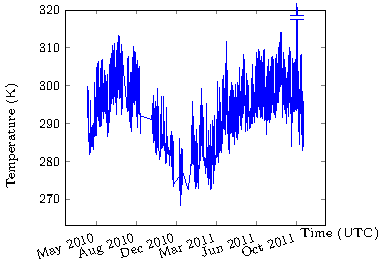
\includegraphics{fig_exemple_original.pdf}
  \caption{Example of a temperature time series data}
  \label{fig:exemple:original}
\end{figure}

\emph{Schema}. We design a \acro{MTSDB} that stores a multiresolution
time series with high resolution at recent times and with low
resolution at older times. The schema is illustrated in the
Figure~\ref{fig:exemple:window}. At the top there are four discs with
different number of measures and at the bottom there is a timeline
showing the resolution subseries along time. Going from most to least
granularity, disks are configured as follows: (i) a measure every 5 h
in the fourth disc which has a capacity of 24 measures and thus it
spans 5 days; (ii) a measure every 2 days in the third disc, with a
capacity of 20 thus spanning 40 days; (iii) a measure every 15 days in
the second disc, with a capacity of 12 thus spanning 180 days and;
(iv) a measure every 50 days in the first disc that, with a capacity
of 12 results in a span of 600 days. This last span is longer than the
original time series so that at least one resolution keeps some data
along the complete original time interval.

\begin{figure}[tp]
  \centering
  \setlength{\unitlength}{1.3mm}
  %%mrd.afegeix_disc(h5,24,mitjana,zero)
%mrd.afegeix_disc(d2,20,mitjana,zero)
%mrd.afegeix_disc(d15,12,mitjana,zero)
%mrd.afegeix_disc(d50,12,mitjana,zero)
\tiny
\begin{center}
%\begin{multicols}{4} 


    \begin{picture}(14,12)(-7,-6)
    \put(0,-1){\makebox(0,0)[c]{{\color{blue}50 days}}}
      \put(0,0){\circle{10}}
      \put(5,0){\circle{0.8}}
      \put(4.33,2.5){\circle{0.8}}
      \put(2.5,4.33){\circle{0.8}}
      \put(0,5){\circle{0.8}}
      \put(-2.5,4.33){\circle{0.8}}   
      \put(-4.33,2.5){\circle{0.8}}
      \put(-5,0){\circle{0.8}}
      \put(-4.33,-2.5){\circle{0.8}}
      \put(-2.5,-4.33){\circle{0.8}} 
      \put(0,-5){\circle{0.8}}
      \put(2.5,-4.33){\circle{0.8}} 
      \put(4.33,-2.5){\circle{0.8}}
      \put(0,0){\vector(0,1){5}}
      \put(0,0){\oval(5,5)[t]}
      \put(-2.5,0){\makebox(0,0)[c]{$\vee$}}
    \end{picture}
%
    \begin{picture}(14,12)(-7,-6)
    \put(0,-1){\makebox(0,0)[c]{{\color{brown}15 days}}}
      \put(0,0){\circle{10}}
      \put(5,0){\circle{0.8}}
      \put(4.33,2.5){\circle{0.8}}
      \put(2.5,4.33){\circle{0.8}}
      \put(0,5){\circle{0.8}}
      \put(-2.5,4.33){\circle{0.8}}   
      \put(-4.33,2.5){\circle{0.8}}
      \put(-5,0){\circle{0.8}}
      \put(-4.33,-2.5){\circle{0.8}}
      \put(-2.5,-4.33){\circle{0.8}} 
      \put(0,-5){\circle{0.8}}
      \put(2.5,-4.33){\circle{0.8}} 
      \put(4.33,-2.5){\circle{0.8}}
      \put(0,0){\vector(0,1){5}}
      \put(0,0){\oval(5,5)[t]}
      \put(-2.5,0){\makebox(0,0)[c]{$\vee$}}
    \end{picture}
%
    \begin{picture}(14,12)(-7,-6)
    \put(0,-1){\makebox(0,0)[c]{{\color{red}2 days}}}
      \put(0,0){\circle{10}}
      %\put(5,0){\circle{0.8}}
      \put(4.82,1.29){\circle{0.8}}
      \put(4.33,2.5){\circle{0.8}}
     \put(3.5,3.5){\circle{0.8}}
      \put(2.5,4.33){\circle{0.8}}
      \put(1.29,4.82){\circle{0.8}}
      %\put(0,5){\circle{0.8}}
      \put(-1.29,4.82){\circle{0.8}}
      \put(-2.5,4.33){\circle{0.8}}
       \put(-3.5,3.5){\circle{0.8}} 
      \put(-4.33,2.5){\circle{0.8}}
    \put(-4.82,1.29){\circle{0.8}}
      %\put(-5,0){\circle{0.8}}
    \put(-4.82,-1.29){\circle{0.8}}
      \put(-4.33,-2.5){\circle{0.8}}
      \put(-3.5,-3.5){\circle{0.8}} 
      \put(-2.5,-4.33){\circle{0.8 } } 
      \put(-1.29,-4.82){\circle{0.8 }}
      % \put(0,-5){\circle{0.8 }}
     \put(1.29,-4.82){\circle{0.8 }}
      \put(2.5,-4.33){\circle{0.8}}
      \put(3.5,-3.5){\circle{0.8}} 
      \put(4.33,-2.5){\circle{0.8}}
  \put(4.82,-1.29){\circle{0.8}}
      \put(0,0){\vector(0,1){5}}
      \put(0,0){\oval(5,5)[t]}
      \put(-2.5,0){\makebox(0,0)[c]{$\vee$}}
    \end{picture}
%
    \begin{picture}(14,12)(-7,-6)
    \put(0,-1){\makebox(0,0)[c]{{\color{cyan}5 hours}}}
      \put(0,0){\circle{10}}
      \put(5,0){\circle{0.8}}
      \put(4.82,1.29){\circle{0.8}}
      \put(4.33,2.5){\circle{0.8}}
     \put(3.5,3.5){\circle{0.8}}
      \put(2.5,4.33){\circle{0.8}}
      \put(1.29,4.82){\circle{0.8}}
      \put(0,5){\circle{0.8}}
      \put(-1.29,4.82){\circle{0.8}}
      \put(-2.5,4.33){\circle{0.8}}
       \put(-3.5,3.5){\circle{0.8}} 
      \put(-4.33,2.5){\circle{0.8}}
    \put(-4.82,1.29){\circle{0.8}}
      \put(-5,0){\circle{0.8}}
    \put(-4.82,-1.29){\circle{0.8}}
      \put(-4.33,-2.5){\circle{0.8}}
      \put(-3.5,-3.5){\circle{0.8}} 
      \put(-2.5,-4.33){\circle{0.8 } } 
      \put(-1.29,-4.82){\circle{0.8 }}
\put(0,-5){\circle{0.8 }}
     \put(1.29,-4.82){\circle{0.8 }}
      \put(2.5,-4.33){\circle{0.8}}
      \put(3.5,-3.5){\circle{0.8}} 
      \put(4.33,-2.5){\circle{0.8}}
  \put(4.82,-1.29){\circle{0.8}}
      \put(0,0){\vector(0,1){5}}
      \put(0,0){\oval(5,5)[t]}
      \put(-2.5,0){\makebox(0,0)[c]{$\vee$}}
    \end{picture}


%\end{multicols}

\vspace{-10pt}

\setlength{\unitlength}{900sp}
\begin{picture}(14460,5066)(7322,-7148)
\thinlines
{\color[rgb]{0,0,0}\put(7300,-6271){\line( 0,-1){386}}
}%
{\color[rgb]{0,0,0}\put(7782,-6271){\line( 0,-1){386}}
}%
{\color[rgb]{0,0,0}\put(8263,-6271){\line( 0,-1){386}}
}%
{\color[rgb]{0,0,0}\put(8745,-6271){\line( 0,-1){386}}
}%
{\color[rgb]{0,0,0}\put(9227,-6271){\line( 0,-1){386}}
}%
{\color[rgb]{0,0,0}\put(9709,-6271){\line( 0,-1){386}}
}%
{\color[rgb]{0,0,0}\put(10191,-6271){\line( 0,-1){386}}
}%
{\color[rgb]{0,0,0}\put(10673,-6271){\line( 0,-1){386}}
}%
{\color[rgb]{0,0,0}\put(11155,-6271){\line( 0,-1){386}}
}%
{\color[rgb]{0,0,0}\put(11637,-6271){\line( 0,-1){386}}
}%
{\color[rgb]{0,0,0}\put(12119,-6271){\line( 0,-1){386}}
}%
{\color[rgb]{0,0,0}\put(12600,-6271){\line( 0,-1){386}}
}%
{\color[rgb]{0,0,0}\put(13082,-6271){\line( 0,-1){386}}
}%
{\color[rgb]{0,0,0}\put(13564,-6271){\line( 0,-1){386}}
}%
{\color[rgb]{0,0,0}\put(14046,-6271){\line( 0,-1){386}}
}%
{\color[rgb]{0,0,0}\put(14528,-6271){\line( 0,-1){386}}
}%
{\color[rgb]{0,0,0}\put(15010,-6271){\line( 0,-1){386}}
}%
{\color[rgb]{0,0,0}\put(15492,-6271){\line( 0,-1){386}}
}%
{\color[rgb]{0,0,0}\put(15974,-6271){\line( 0,-1){386}}
}%
{\color[rgb]{0,0,0}\put(16456,-6271){\line( 0,-1){386}}
}%
{\color[rgb]{0,0,0}\put(16938,-6271){\line( 0,-1){386}}
}%
{\color[rgb]{0,0,0}\put(17419,-6271){\line( 0,-1){386}}
}%
{\color[rgb]{0,0,0}\put(17901,-6271){\line( 0,-1){386}}
}%
{\color[rgb]{0,0,0}\put(18383,-6271){\line( 0,-1){386}}
}%
{\color[rgb]{0,0,0}\put(18865,-6271){\line( 0,-1){386}}
}%
{\color[rgb]{0,0,0}\put(19347,-6271){\line( 0,-1){386}}
}%
{\color[rgb]{0,0,0}\put(19829,-6271){\line( 0,-1){386}}
}%
{\color[rgb]{0,0,0}\put(20311,-6271){\line( 0,-1){386}}
}%
{\color[rgb]{0,0,0}\put(20793,-6271){\line( 0,-1){386}}
}%
{\color[rgb]{0,0,0}\put(21275,-6271){\line( 0,-1){386}}
}%
{\color[rgb]{0,0,0}\put(7300,-6271){\line( 0,-1){1157}}
}%
{\color[rgb]{0,0,0}\put(9709,-6271){\line( 0,-1){1157}}
}%
{\color[rgb]{0,0,0}\put(12119,-6271){\line( 0,-1){1157}}
}%
{\color[rgb]{0,0,0}\put(14528,-6271){\line( 0,-1){1157}}
}%
{\color[rgb]{0,0,0}\put(16938,-6271){\line( 0,-1){1157}}
}%
{\color[rgb]{0,0,0}\put(19347,-6271){\line( 0,-1){1157}}
}%
{\color[rgb]{0,0,0}\put(21756,-6271){\line( 0,-1){1157}}
}%
{\color[rgb]{0,0,0}\put(7300,-6271){\line( 1, 0){14456}}
}%

\put(7322,-6271){\line( 0,1){3000}}
\put(21756,-7783){\makebox(0,0)[b]{now}}%
\put(7322,-7783){\makebox(0,0)[b]{600 days back}}%

\color{blue}
\put(21782,-5928){\line( -1,0){14460}}
\put(21782,-5928){\line( 0,1){779}}
\put(21782,-5149){\line( -1,0){14460}}
\put(7322,-5928){\line( 0,1){779}}
\put(14530,-5450){\makebox(0,0)[c]{600 days}}

\color{brown}
\put(21782,-5149){\line( 0,1){779}}
\put(21782,-4370){\line( -1,0){4438}}
\put(17344,-5149){\line( 0,1){779}}
\put(19563,-4800){\makebox(0,0)[c]{180 days}}

\color{red}
\put(21782,-4370){\line( 0,1){779}}
\put(21782,-3591){\line( -1,0){964}}
\put(20818,-4370){\line( 0,1){779}}
\put(21300,-3950){\makebox(0,0)[c]{40d}}

\color{cyan}
\put(21782,-3591){\line( 0,1){779}}
\put(21782,-2812){\line( -1,0){120}}
\put(21661,-3591){\line( 0,1){779}}
\put(21300,-3201){\makebox(0,0)[c]{5d}}
\end{picture}%


\normalsize

\end{center}
  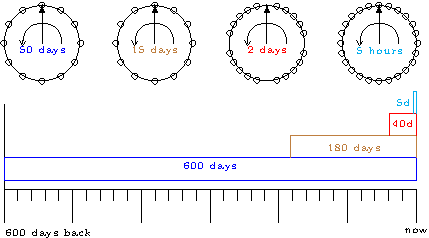
\includegraphics{fig_exemple_window.pdf}
  \caption{Schema of multiresolution}
  \label{fig:exemple:window}
\end{figure}

\emph{Attribute aggregate functions}.  In order to illustrate this
example we consolidate all the resolution subseries using the
mean$^\zohe{}$ aggregate function and the two highest resolution
subseries using the maximum$^\zohe{}$ aggregate function. 



\emph{Consolidation}. The time subseries after consolidating the
\acro{MTSDB} are shown in the Figure~\ref{fig:exemple:4mrd}, where
each graphic corresponds to the possible $\seriedisc$ queries, that is
every resolution disc time series from the \acro{MTSDB}. Each title
shows the resolution subseries and its cardinal, and each attribute
aggregate function has different colour.  Each time series is plotted
with \zohe{} representation function $S(t)^\zohe{}$. Time axis has
\acro{UTC} units rounded to nearest time points and temperature axis
has Kelvin units. Outlayers are marked as discontinuities, for
instance see fourth plot's 2938 K maximum.

\begin{figure}[tp]
  \centering
  % \tikzset{
  %   every picture/.style={scale=0.7},
  % }
  % 
  \begin{tikzpicture}[scale=0.6, every node/.style={transform shape}]
    \begin{axis}[
        multiresoluciodate,
        title={$R_1$: 5h $|24|$},
        xticklabel={\day--\hour:\minute},
        clip=false,
        ]
       \addplot[const plot mark right, blue] table[col sep=comma] {imatges/exemple/dades-matriu0/R18000mean_zohe.csv};
     \node[left] at (axis cs:2011-10-19,274) {\footnotesize oct.~2011};
  \end{axis}
\end{tikzpicture}
%
  \begin{tikzpicture}[scale=0.6, every node/.style={transform shape}]
    \begin{axis}[
        multiresoluciodate,
        title={$R_2$: 2d $|20|$},
        xticklabel={\day~\pgfcalendarmonthshortname{\month}},
        clip=false,
        ]
       \addplot[const plot mark right, blue] table[col sep=comma] {imatges/exemple/dades-matriu0/R172800mean_zohe.csv};
     \node[left] at (axis cs:2011-10-21,279) {\footnotesize 2011};
  \end{axis}
\end{tikzpicture}
%
  \begin{tikzpicture}[scale=0.6, every node/.style={transform shape}]
    \begin{axis}[
        multiresoluciodate,
        title={$R_3$: 15d $|12|$},
        xticklabel={\day~\pgfcalendarmonthshortname{\month}},
        y filter/.code = { \pgfmathparse{(#1>320)*330+(#1<320)*#1}},
        ymax = 320,
        clip=false,
        ]

       \addplot[const plot mark right, blue] table[col sep=comma] {imatges/exemple/dades-matriu0/R1296000mean_zohe.csv};

      \addplot[const plot mark right, orange] table[col sep=comma] {imatges/exemple/dades-matriu0/R1296000maximum_zohe.csv};

      \node[right] at (axis cs:2011-10-07,330) {\footnotesize(2938)};
       \node (break) at (axis cs:2011-09-23,325)[inner sep=0pt,minimum width=0.75em, minimum height=0.5ex,fill=white] {};
    \draw [fill=red,color=orange] (break.north east) -- (break.north west) (break.south west) -- (break.south east);

     \node[left] at (axis cs:2011-10-27,273) {\footnotesize 2011};

  \end{axis}
\end{tikzpicture}
%
\begin{tikzpicture}[scale=0.6, every node/.style={transform shape}]
    \begin{axis}[
        multiresoluciodate,
        xticklabel={\pgfcalendarmonthshortname{\month}~\year},
        title={$R_4$: 50d $|12|$},
        xlabel={Temps (UTC)},
%        ylabel={Temperatura (K)},
        ymax = 320,
        clip=false,
%v1.6     restrict y to domain=0:320,
        y filter/.code = { \pgfmathparse{(#1>320)*330+(#1<320)*#1}},
        ]

       \addplot[const plot mark right, blue] table[col sep=comma] {imatges/exemple/dades-matriu0/R4320000mean_zohe.csv};
       \addlegendentry{mitjana};

       \addplot[const plot mark right, orange] table[col sep=comma] {imatges/exemple/dades-matriu0/R4320000maximum_zohe.csv};
       \addlegendentry{màxim};

       \node[right] at (axis cs:2011-10-12,330) {\footnotesize(2938)};
       \node (break) at (axis cs:2011-08-24,325)[inner sep=0pt,minimum width=0.75em, minimum height=0.5ex,fill=white] {};
    \draw [fill=red,color=orange] (break.north east) -- (break.north west) (break.south west) -- (break.south east);

  \end{axis}
\end{tikzpicture}




%%% Local Variables:
%%% TeX-master: "../../main"
%%% End:

  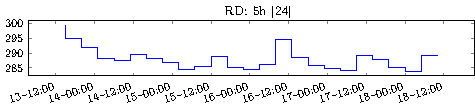
\includegraphics{fig_exemple_4mrd1.pdf}
  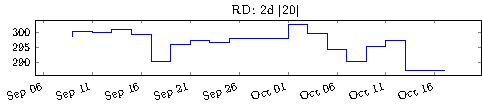
\includegraphics{fig_exemple_4mrd2.pdf}
  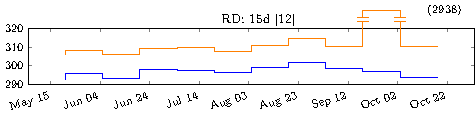
\includegraphics{fig_exemple_4mrd3.pdf}
  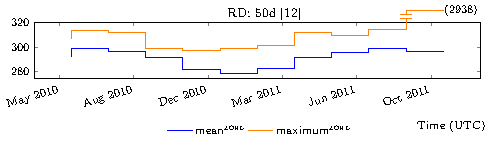
\includegraphics{fig_exemple_4mrd4.pdf}
  \caption{Resolution subseries in the MTSDB}
  \label{fig:exemple:4mrd}
\end{figure}

In all the four plots, we can see that mean aggregate function has
filled missing data and filtered outlayer observations. This is due
to the aggregate function coming from a \zohe{} interpretation.

Figure~\ref{fig:exemple:4mrdtot} shows the $\totalseries$
queries for the mean$^{\zohe}$ aggregate function resolution and for
the maximum$^{\zohe}$ resolution.  Each resulting time series is
plotted interpolating linearly its measures, note that this linearly
visualisation seems right time displaced as time series comes from a
\zohe{} aggregation.  Comparing this figure with the original series
in Figure~\ref{fig:exemple:original}, we observe that it resembles an
incremental low-pass filter because we applied mean aggregation while
the maximum aggregation resembles an envelope function.

%\tikzsetnextfilename{fig_exemple_4mrdtot}
\begin{figure}[tp]
  \centering
  %\tikzset{every picture/.style={scale=0.8}}
  %\usetikzlibrary{dateplot}  
%\usetikzlibrary{pgfplots.groupplots}

\pgfplotsset{
   petit/.style={
        ylabel=Temperature (K),
%        width=\textwidth,
%        height=3.5cm,
        legend style={font=\footnotesize},
        tick label style={font=\footnotesize},
        label style={font=\tiny},
        title style={font=\small,below, anchor=north,fill=white},
        xticklabel style= {rotate=15,anchor=east},
%        every axis title shift=0pt,
%        max space between ticks=15,
        every mark/.append style={mark size=6},
        major tick length=0.1cm,
        minor tick length=0.066cm,
        very thin,
        every axis legend/.append style={
          at={(1,0.02)},
          anchor=south east,
          draw = none},
        legend columns = 4,
    }
}

\begin{tikzpicture}
    \begin{axis}[
        petit,
        date coordinates in=x,
        xticklabel={\pgfcalendarmonthshortname{\month} \year},
        xlabel=Time (UTC),
%        unbounded coords=jump, %v>1.4
%        unbounded coords=discard, %v>1.4
        ymax = 320,
        clip=false,
%v1.6     restrict y to domain=0:320,
        y filter/.code = { \pgfmathparse{(#1>320)*330+(#1<320)*#1}},
        ]

       \addplot[black!15] file {dades/matriu0.originalbyday.dat};
       \addlegendentry{original};

       \addplot[blue] table[col sep=comma] {dades/mrdb-matriu0/union1.csv};
       \addlegendentry{mean};

       \addplot[orange] table[col sep=comma] {dades/mrdb-matriu0/union0.csv};
       \addlegendentry{max};

%       \node[right] at (axis cs:2011-10-12,330) {\mbox{(2938)}};
       \node (break) at (axis cs:2011-09-25,325)[inner sep=0pt,minimum width=0.9em, minimum height=0.4ex,fill=white] {};
    \draw [fill=red,color=orange] (break.north east) -- (break.north west) (break.south west) -- (break.south east);


  \end{axis}
\end{tikzpicture}
%http://tex.stackexchange.com/questions/46422/axis-break-in-pgfplots

%http://tex.stackexchange.com/questions/52409/insert-a-separate-mark-inside-a-pgfplots-graph



%%% Local Variables:
%%% TeX-master: "../main"
%%% ispell-local-dictionary: "british"
%%% End:

  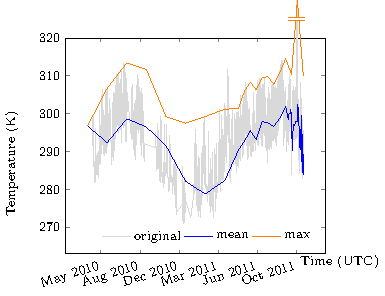
\includegraphics{fig_exemple_4mrdtot.pdf}
  \caption{$\totalseries$ for the mean$^{\zohe}$ and maximum$^{\zohe}$
    resolutions}
  \label{fig:exemple:4mrdtot}
\end{figure}


In conclusion, this \acro{MTSDB} example schema does not store the
complete original data but a compression of the original function
which contains more data for recent times.  Each of the
$\seriedisc$ time series is regular with $\delta$. Although
$\totalseries$ is not a regular time series, it has piece-wise
regularity as a concatenation of every disc's $\delta$.  The purpose
of this example is to show how the multiresolution is computed for a
time series, it has been computed offline as the original data had
already been acquired. However, a \acro{MTSMS} is designed to
consolidate while the original data is being acquired so that the
multiresolution computation spreads along the acquisition and the
computing time becomes less critical.


%%% Local Variables:
%%% TeX-master: "main"
%%% ispell-local-dictionary: "british"
%%% End:

% LocalWords:  multiresolution MTSDB


%related work, conclusion, acknowledgement
\section{Related Work}

The research in time series data management has increased last decade
as the procedure of processing and synthesizing information becomes
complicated if data varies over time. From this point of view we focus
on DBMS aimed to time series where we find two main perspectives in
current research.


On the one hand, there are DBMS with some properties and operations
for time series.

RRDtool from Oetiker \cite{rrdtool} is a professional database
management system extremely used by the free software community. It is
used in professional monitoring systems and its efficiency and speed
when processing time series is being improved. Nevertheless, it is
focused to a particular kind of data, gauges and counters, and it has
not general time series operations.

Cougar \cite{bonnet01} is a sensor database system. It has two
structures: one for sensor properties stored into relations and
another for time series stored into data sequences from sensors.  Time
series have specific operations and can combine relations and
sequences.


SciDB \cite{stonebraker09:scidb} and SciQL \cite{zhang11} are array
database systems. These systems are intended for science applications,
in which time series play a principal role. They structure time series
into arrays in order to achieve multidimensional analysis.



On the other hand, there is the relational DBMS model as the common
study for DBMS theories. The relational DBMS model is continuously
evolving \cite{date:thethirdmanifesto}.

Particularly regarding time data,
intensive research has been carried in the bitemporal data field, that
is the management of history using time intervals.  The recent
temporal data research in relational DBMS model terms
\cite{date02:_tempor_data_relat_model} marks a promising
foundation. It models bitemporal data as relations extended with time
intervals attributes and extends relational operations in order to
deal with related time aspects.

Although bitemporal data and time series data are not exactly the same
and so can not be treated interchangeably \cite{schmidt95},
time series research can benefit from two aspects of this bitemporal
data research. First, it shows the way to extend relational DBMS with
new types and how to model them. Second, it settles some time-related
concepts that can apply well to time series.






\section{Conclusions} 

In this paper we have shown a MTSMS model, including the requirements
for these special systems and how they can be applied to an example
time series. The main objective is to store compactly a time series
and manage consistently its temporal dimension.

Our MTSMS model proposes to store a time series split into time
subseries, which we call resolution discs.  Each resolution disc has a
different resolution and is compacted with an attribute interpolation
function. Therefore, in a multiresolution database the configuration
parameters are the quantity of resolution discs and the three
parameters associated with each: the consolidation step, the attribute
interpolation function and the capacity.

The data model shown is the first step to develop a complete model for
a MTSMS but in future the operations will be defined. In this context,
there is a need for a model collecting generic properties for the
TSMS, as it can be the time series union operation or the time
interval operations. Then, the multiresolution model would be build
upon the generic TSMS model.

In an example we have shown a possible application of a MTSMS. The
resulting database has the information we have extracted with the
attribute interpolation function. We show that in this example we want
not an approximation to the original function but an extraction of
some interesting information. Then the database is ready to answer
time series questions keeping in mind that it holds this information
summary.



Amb aquesta recerca volem demostrar que l'ús de SGBD per a les sèries temporals facilitarà enormement el treball amb aquestes.
L'interès actual ens fa ser optimistes per aventurar que aviat podrem gestionar les sèries temporals adequadament amb els SGBD.



\section*{Acknowledgements}

This work was supported by Universitat Polit\`{e}cnica de Catalunya (UPC).

Data comes from iSense project \todo{isense}.







%%% Local Variables:
%%% TeX-master: "main"
%%% ispell-local-dictionary: "british"
%%% End:

% LocalWords:  DBMS



\printbibliography{}


\end{document}


%%% Local Variables: 
%%% ispell-local-dictionary: "british"
%%% End: 




%%%%%%%%%%%%%%%%%%%%%%%%%%%%%%%%%%%%%%%%%%%%%%%%%%%%%%%%%%%%%%%%%%%%%%%%%%  
% Model and requirements for a Multiresolution Time Series Database Management System
%
% Copyright (C) 2012 Aleix Llusà Serra, Teresa Escobet Canal, Sebastià Vila-Marta.
% 
% This LaTeX document is free software: you can redistribute it and/or
% modify it under the terms of the GNU General Public License as
% published by the Free Software Foundation, either version 3 of the
% License, or (at your option) any later version.
%
% This document is distributed in the hope that it will be useful, but
% WITHOUT ANY WARRANTY; without even the implied warranty of
% MERCHANTABILITY or FITNESS FOR A PARTICULAR PURPOSE. See the GNU
% General Public License for more details.
%
% You should have received a copy of the GNU General Public License
% along with this document. If not, see <http://www.gnu.org/licenses/>.
%
%
% Aleix Llusà Serra
% Departament de Disseny i Programació de Sistemes Electrònics de la Universitat Politècnica de Catalunya (DiPSE-UPC)
% Escola Politècnica Superior d'Enginyeria de Manresa (EPSEM)
% Av. de les Bases de Manresa, 61-73
% 08242 Manresa (Barcelona)
% PAÏSOS CATALANS 
%
% aleix (a) dipse.upc.edu
% 
% Source LaTeX document code is located at 
% <http://escriny.epsem.upc.edu/projects/rrb/>
%%%%%%%%%%%%%%%%%%%%%%%%%%%%%%%%%%%%%%%%%%%%%%%%%%%%%%%%%%%%%%%%%%%%%%%%%% 